\documentclass[aspectratio=169,10pt]{beamer}\usetheme{default}\usecolortheme{seahorse}\setbeamertemplate{navigation symbols}{}
\usepackage[T1]{fontenc}\usepackage[utf8]{inputenc}\usepackage{helvet}\usepackage{booktabs,amsmath}
\DeclareUnicodeCharacter{2019}{\textquoteright}\DeclareUnicodeCharacter{2013}{--}
\setbeamersize{text margin left=0.6cm,text margin right=0.6cm}\setbeamerfont{frametitle}{size=\large,series=\bfseries}
\setbeamertemplate{footline}{\hfill{\tiny\textcolor{red!70!black}{DRAFT for the author\textquoteright{}s review, v2026-11-21-11-14-34}\quad\insertframenumber}\hspace{1em}\vspace{0.4em}}
\title{Road safety in Côte-des-Neiges--Notre-Dame-de-Grâce}
\subtitle{What the police collision record shows, 2012--2021}
\author{Rick Hoge, PhD}\date{Draft, November 19, 2026 \quad {\footnotesize v2026-11-21-11-14-34}}
\begin{document}
\begin{frame}\titlepage
{\footnotesize The views expressed here are the author's own and do not reflect the position of any institution or organization. Nothing in this document should be considered an engineering opinion or legal advice.}
\end{frame}

\begin{frame}{What the record is, and what it is not}
\begin{itemize}\setlength\itemsep{5pt}
\item \textbf{Source.} Ville de Montréal open data « Collisions routières »: the SPVM's accident reports, January 1, 2012 to December 31, 2021, one row per collision (218{,}272 rows), with a recorded point.
\item \textbf{Only collisions involving a motor vehicle that police attended.} A fall, a bicycle striking a pedestrian, or a collision nobody reported is not in it.
\item \textbf{It ends in 2021.} Nothing here describes a street as it is laid out today.
\item \textbf{No age and no exposure.} The record does not say how many people walked, cycled or drove through a place. \textbf{A count at a place is not a risk}: busy places have long records.
\item \textbf{Location.} The police place most collisions on the nearest intersection. 628 rows placed at a police district's centroid inside the borough (« précision nulle ») are left out of every count here.
\item \textbf{Cyclists and pedestrians are kept apart} throughout: no pooled figure.
\end{itemize}
\end{frame}

\begin{frame}{The borough's record in ten years}
\begin{columns}[T]\begin{column}{0.47\linewidth}
\begin{tabular}{@{}lr@{}}\toprule
Collisions inside the borough & 17{,}182 \\
\quad property damage only & 13{,}800 \\
\quad light injury & 3{,}213 \\
\quad severe injury & 147 \\
\quad fatal & 22 \\\midrule
With a pedestrian victim & 1{,}002 \\
\quad severe or fatal collision & 94 \\
\quad pedestrians killed & 16 \\
Involving a bicycle & 500 \\
\quad severe or fatal collision & 21 \\
\quad cyclists killed & 1 \\
Involving a motorcycle & 190 \\\bottomrule
\end{tabular}
\end{column}\begin{column}{0.5\linewidth}
\begin{itemize}\setlength\itemsep{6pt}
\item 22 people were killed in the borough's 22 fatal collisions; 16 of them were pedestrians.
\item The borough holds 9.0~\% of the collisions recorded in the City's 19 boroughs, 10.3~\% of those with a pedestrian victim and 6.3~\% of those involving a bicycle.
\item It is the City's most populous borough (170{,}583 residents in the 2021 Census, by dissemination area) with 256 km of street.
\item Severity is the collision's own: in a « severe or fatal » collision with a pedestrian victim, the person most hurt is not always the pedestrian.
\end{itemize}
\end{column}\end{columns}
\end{frame}

\begin{frame}{How the borough compares with the rest of Montréal}
\begin{center}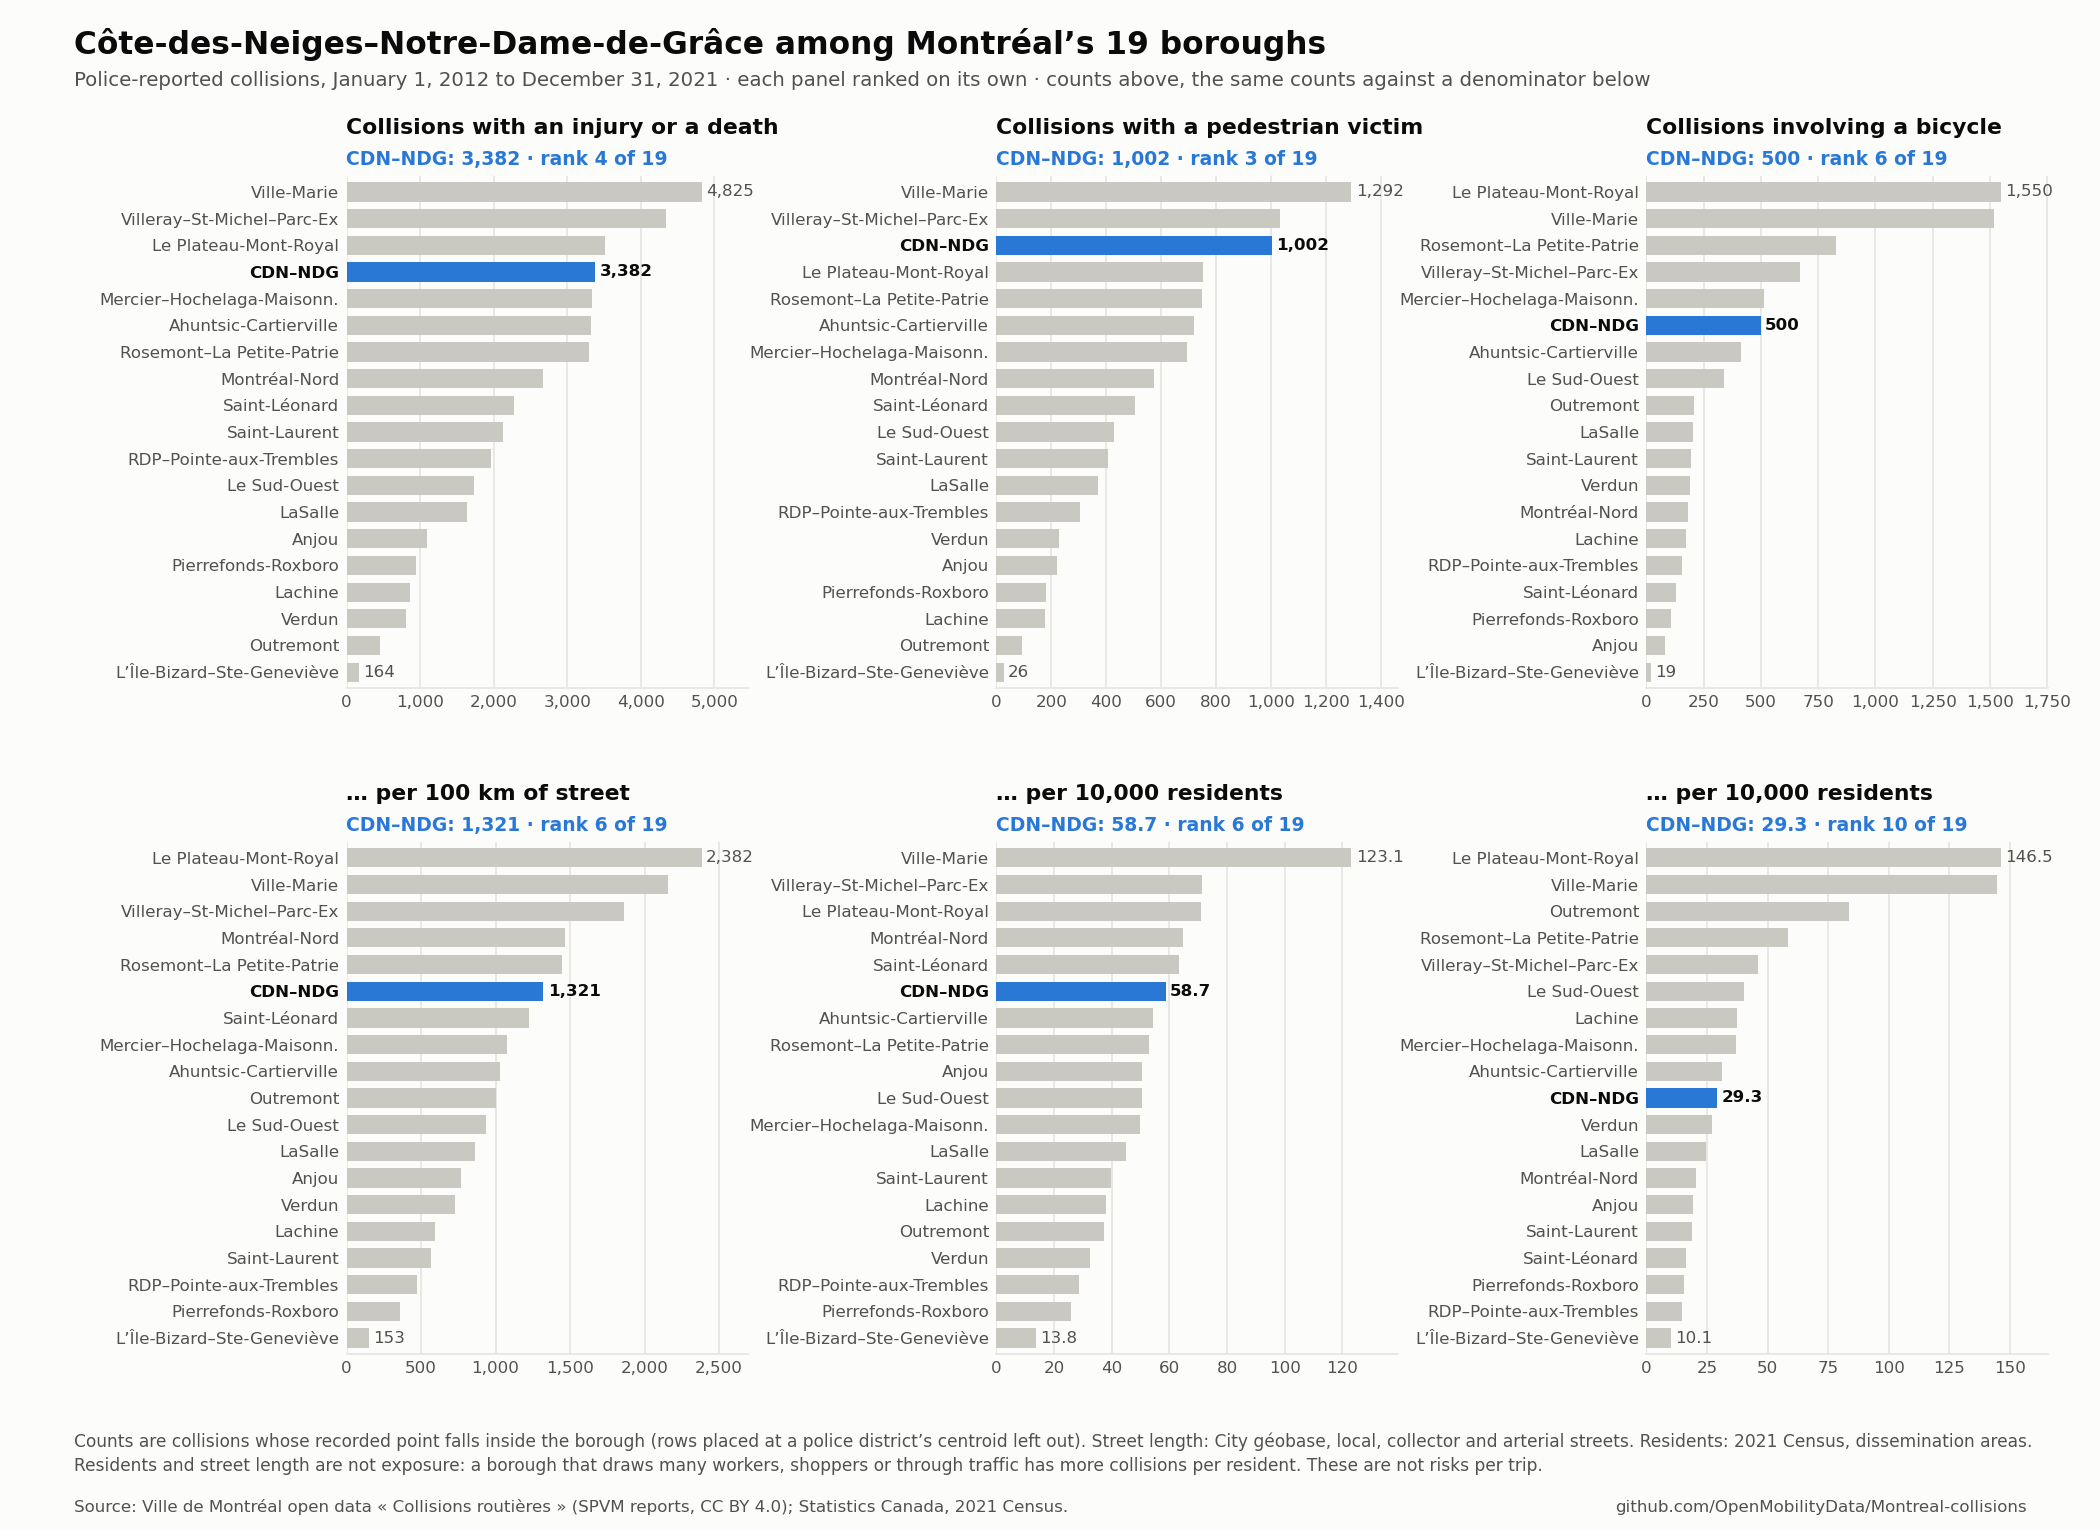
\includegraphics[width=\linewidth,height=0.86\textheight,keepaspectratio]{../derived/figures/borough-comparison/borough_comparison_en.png}\end{center}
\end{frame}

\begin{frame}{Reading the comparison}
\small
\begin{tabular}{@{}lrrr@{}}\toprule
Rank among the 19 boroughs (1 = most) & count & per 100 km of street & per 10,000 residents \\\midrule
Collisions with an injury or a death & 4 & 6 & 13 \\
\quad of which severe or fatal & 3 & 4 & 6 \\
With a pedestrian victim & 3 & & 6 \\
\quad of which severe or fatal & 2 & & 5 \\
Involving a bicycle & 6 & & 10 \\
\quad of which severe or fatal & 5 & & 9 \\\bottomrule
\end{tabular}
\medskip
\begin{itemize}\setlength\itemsep{4pt}
\item By count the borough is near the top because it is the largest. Set against its streets or its residents it moves toward the middle of the 19.
\item \textbf{There is no fair single ranking.} Residents and street length are not exposure: Ville-Marie's counts per resident reflect the people who come downtown, not only those who live there. Nobody has counted trips on foot, by bicycle or by car by borough.
\item A lower bicycle count per resident may mean safer streets or fewer people cycling. The record cannot tell which.
\end{itemize}
\end{frame}

\begin{frame}{Where the collisions are recorded}
\begin{center}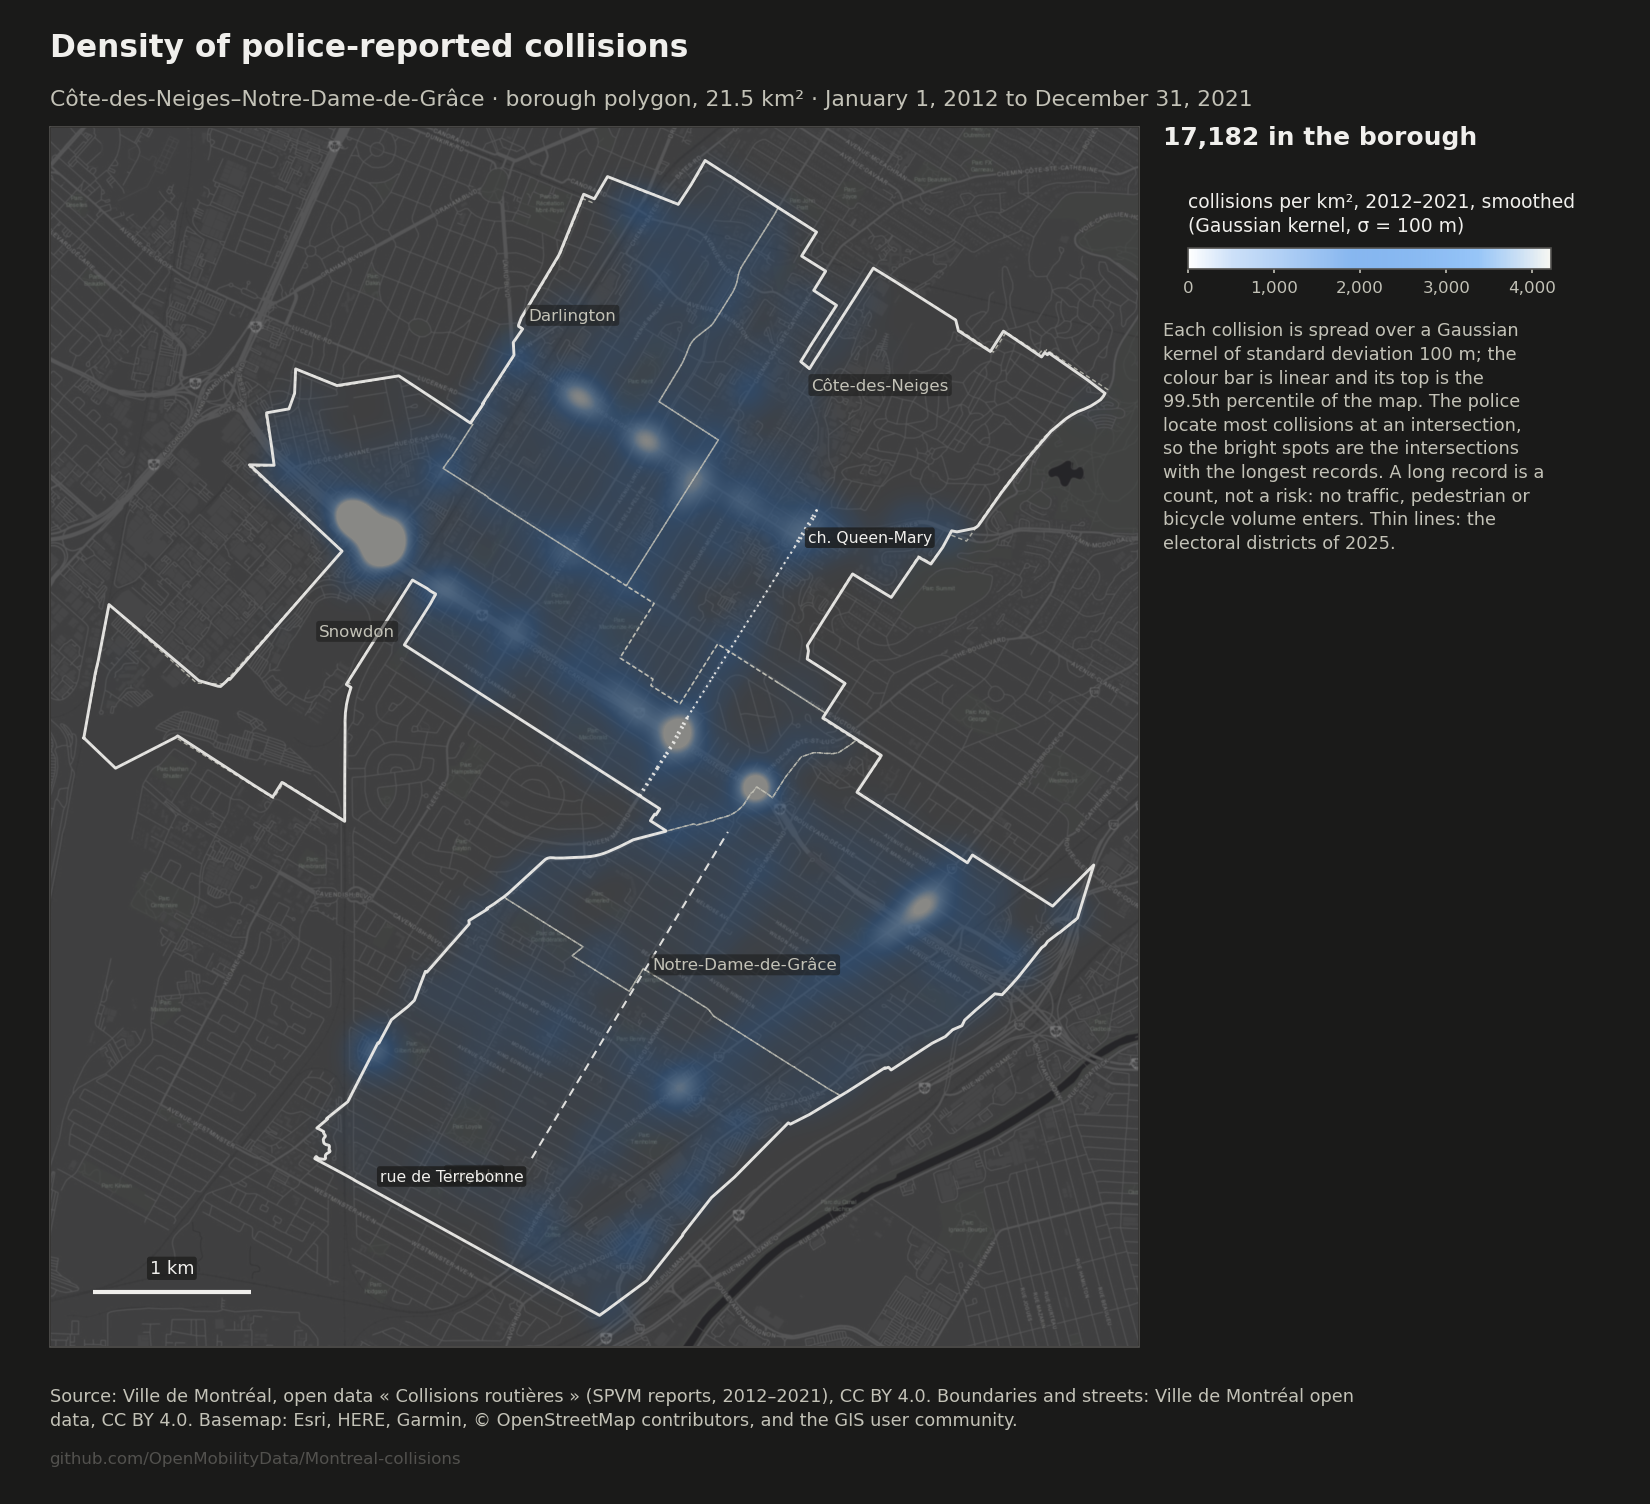
\includegraphics[width=\linewidth,height=0.84\textheight,keepaspectratio]{../derived/figures/cdn-ndg-maps/cdn_ndg_heat_en.png}\end{center}
\end{frame}

\begin{frame}{By electoral district}
\begin{center}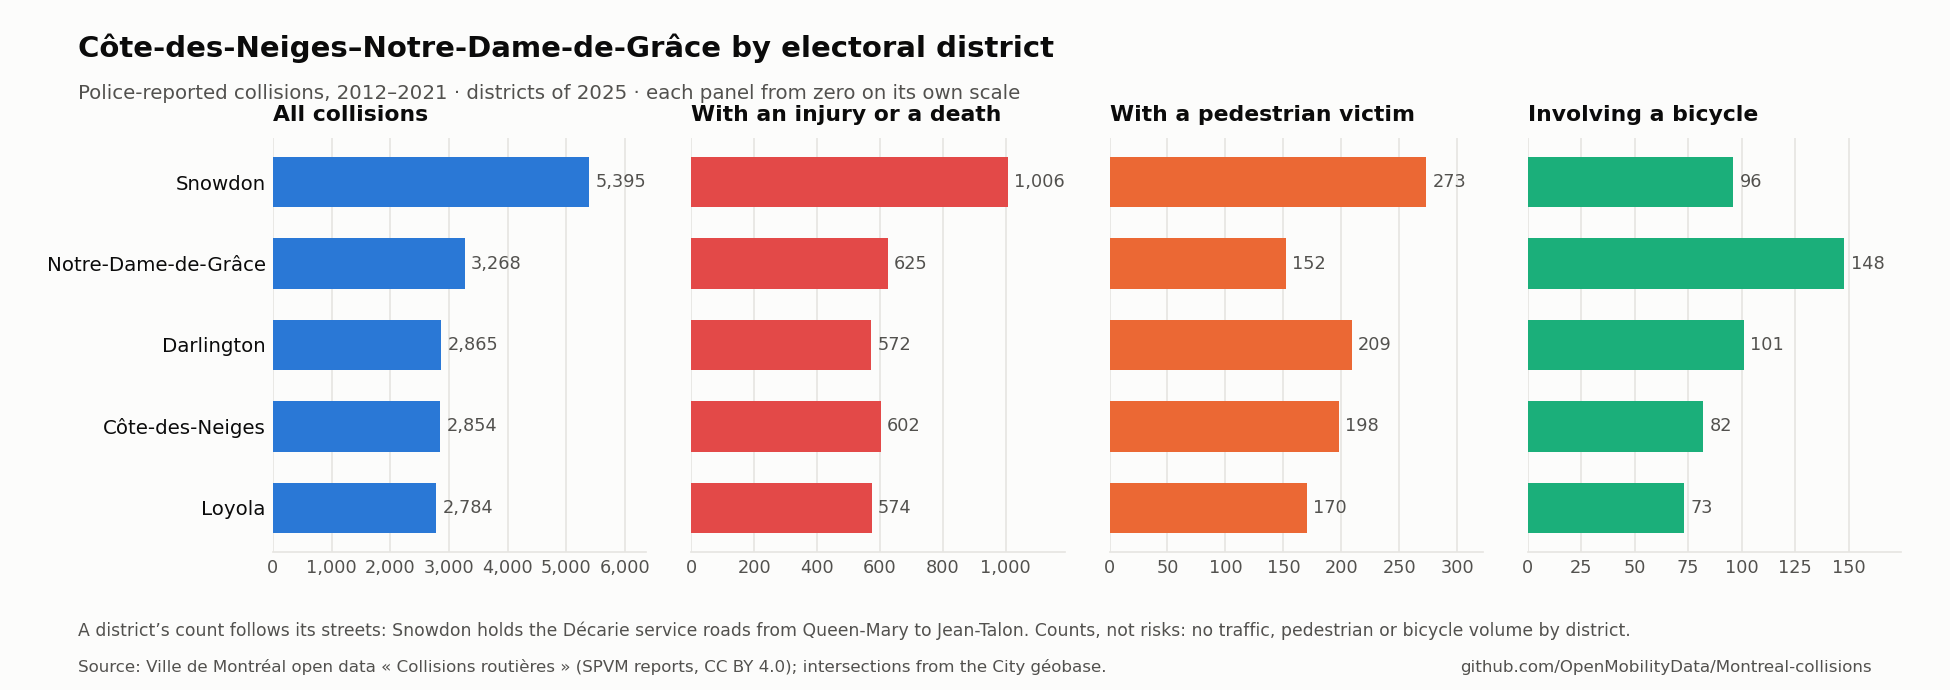
\includegraphics[width=\linewidth,height=0.8\textheight,keepaspectratio]{../derived/figures/cdn-ndg-charts/cdn_ndg_districts_en.png}\end{center}
\end{frame}

\begin{frame}{By year}
\begin{center}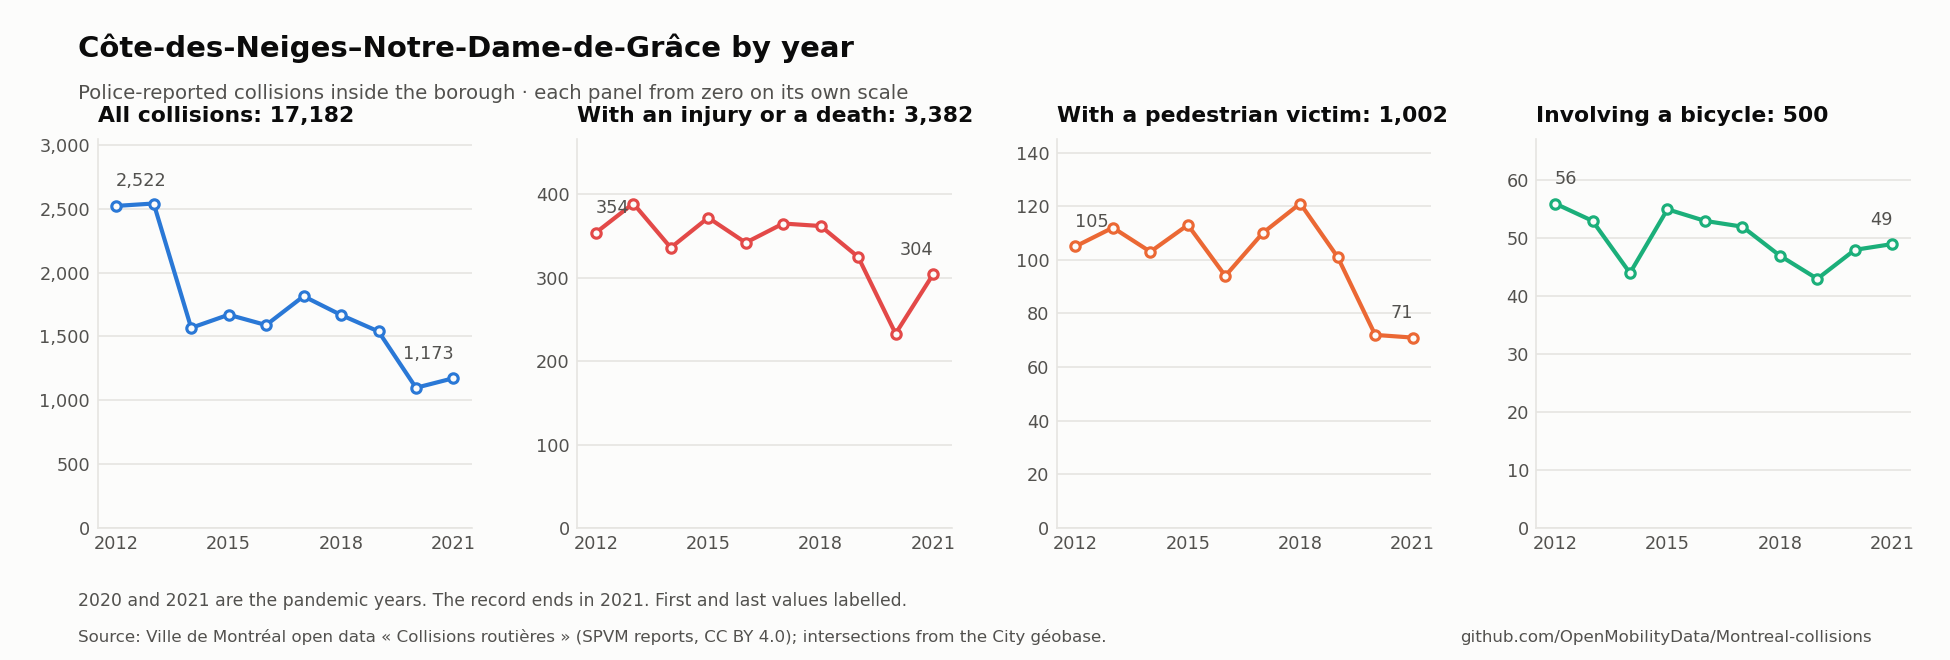
\includegraphics[width=\linewidth,height=0.8\textheight,keepaspectratio]{../derived/figures/cdn-ndg-charts/cdn_ndg_yearly_en.png}\end{center}
\end{frame}

\begin{frame}{Pedestrians: where the collisions are recorded}
\begin{center}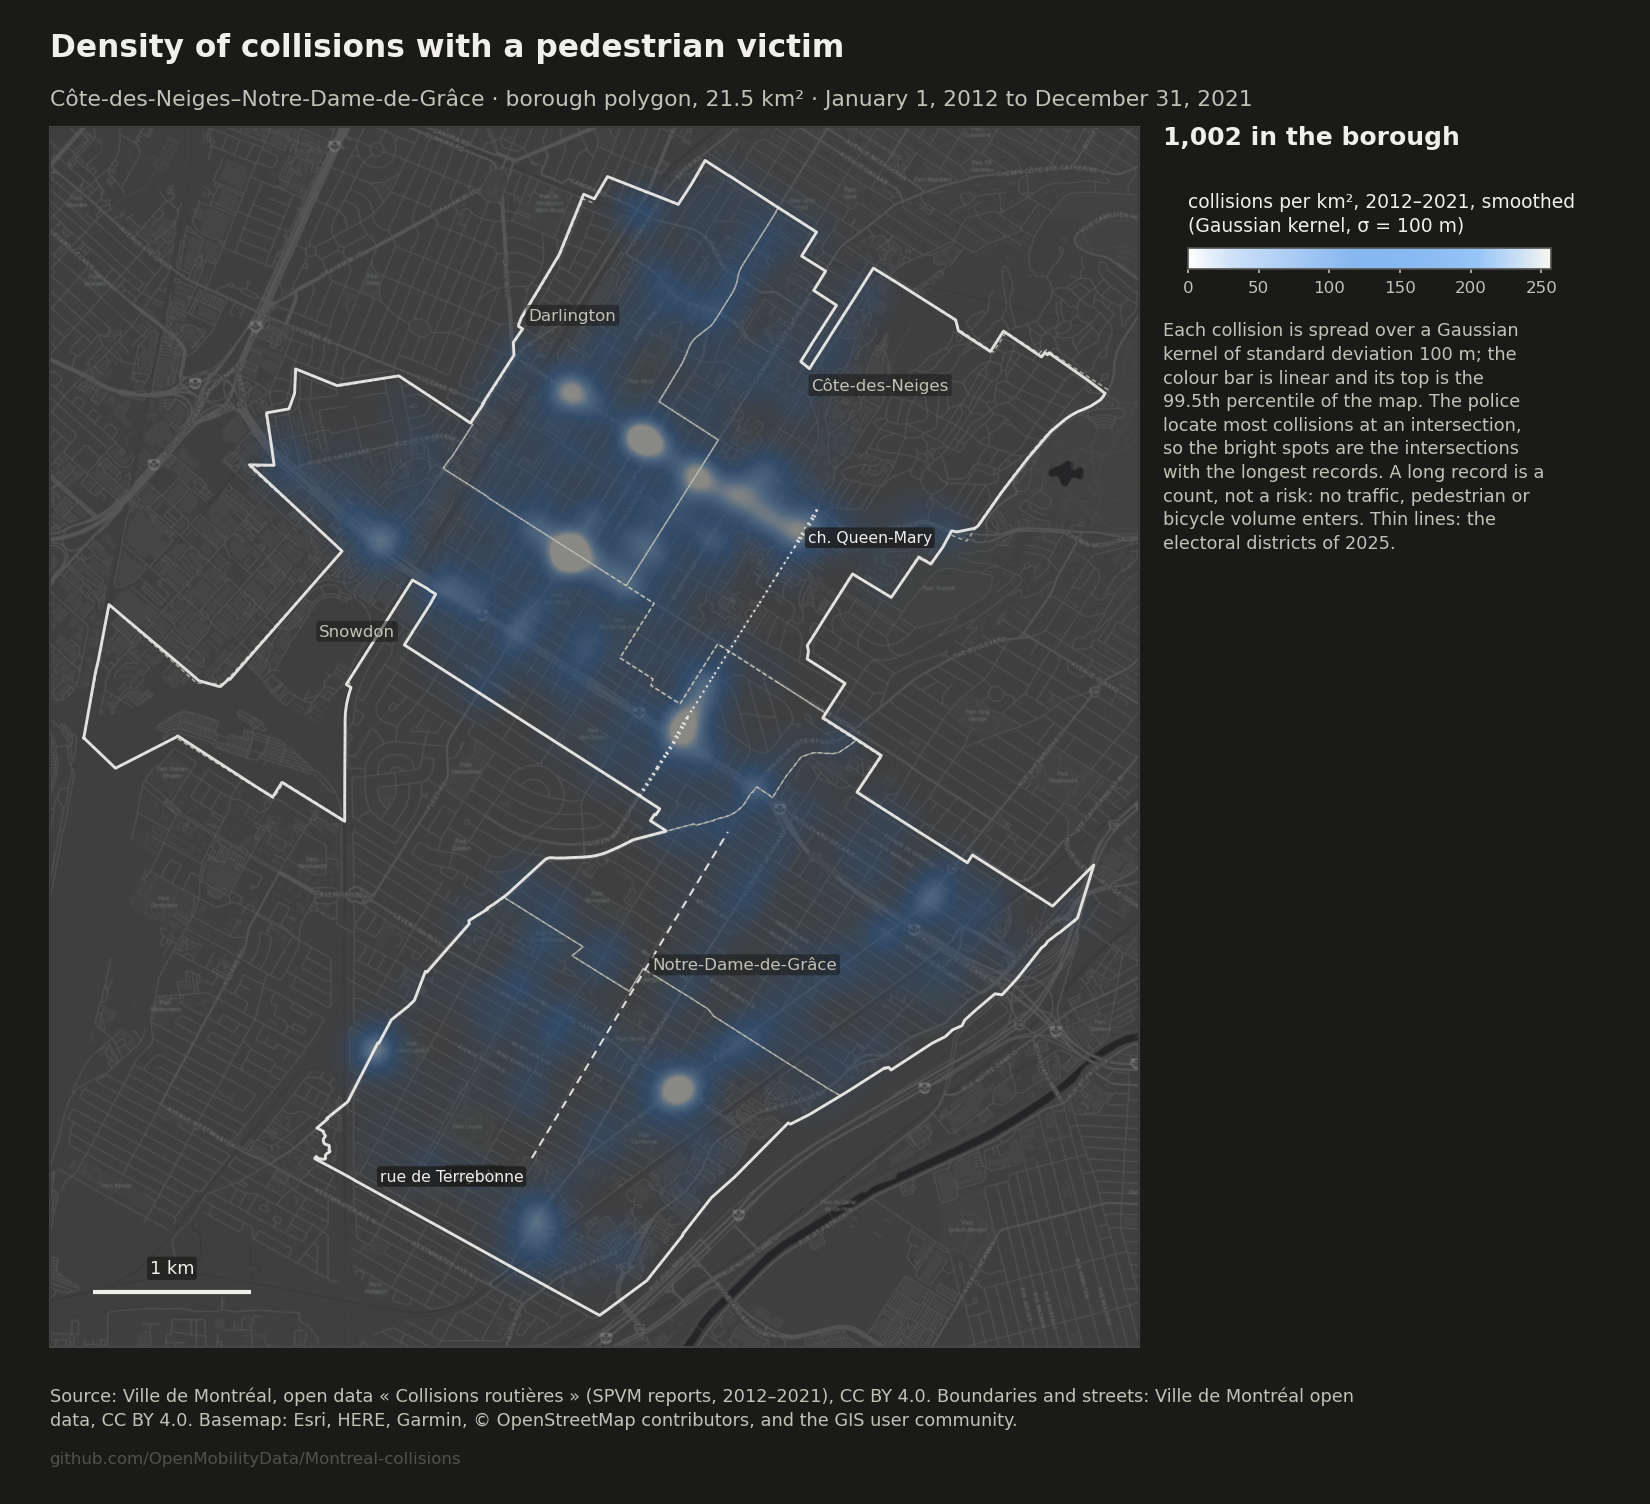
\includegraphics[width=\linewidth,height=0.84\textheight,keepaspectratio]{../derived/figures/cdn-ndg-maps/cdn_ndg_ped_heat_en.png}\end{center}
\end{frame}

\begin{frame}{Pedestrians: collisions with a death or a severe injury}
\begin{center}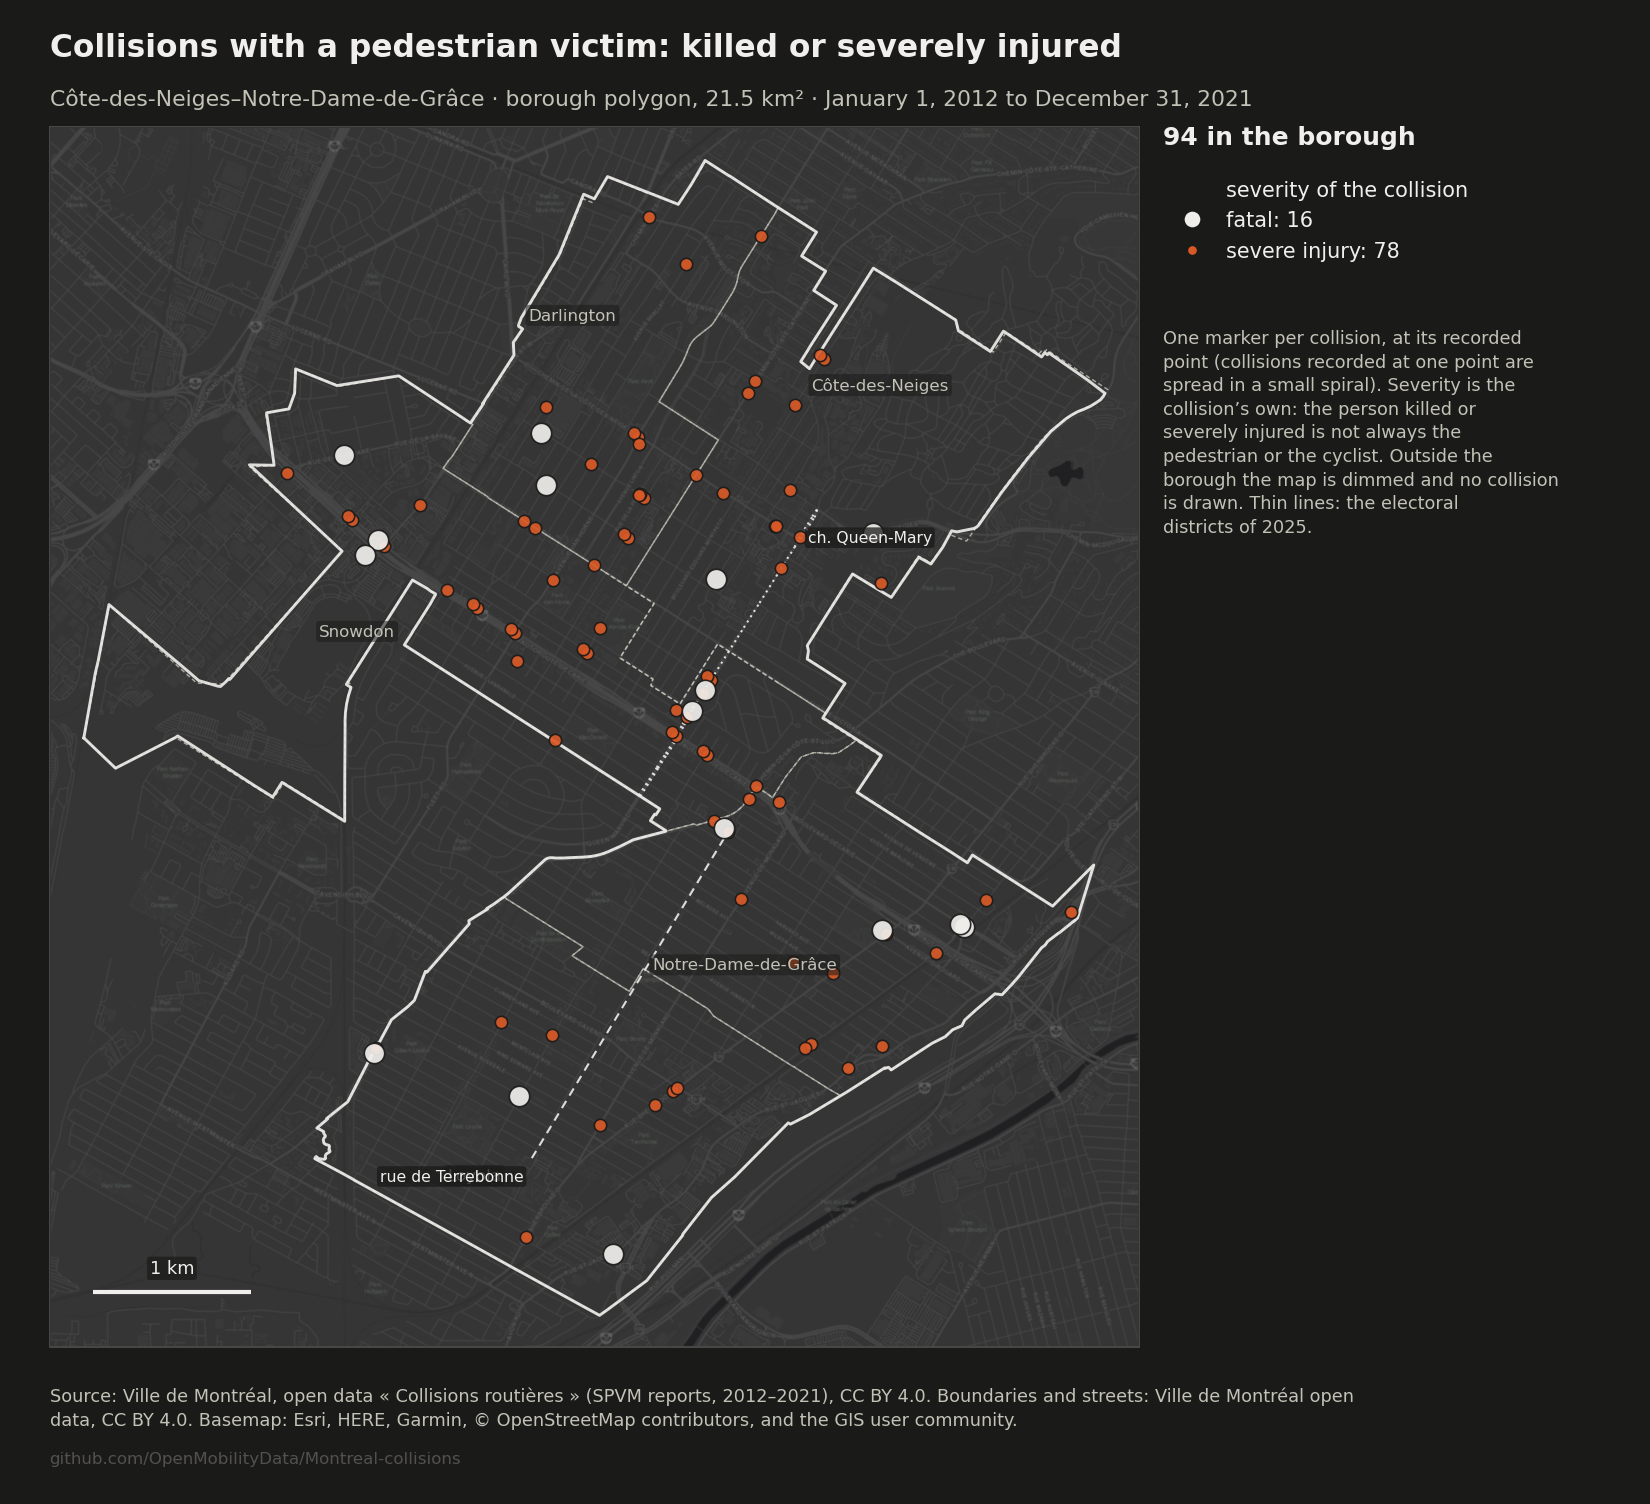
\includegraphics[width=\linewidth,height=0.84\textheight,keepaspectratio]{../derived/figures/cdn-ndg-maps/cdn_ndg_ped_serious_en.png}\end{center}
\end{frame}

\begin{frame}{Bicycles: where the collisions are recorded}
\begin{center}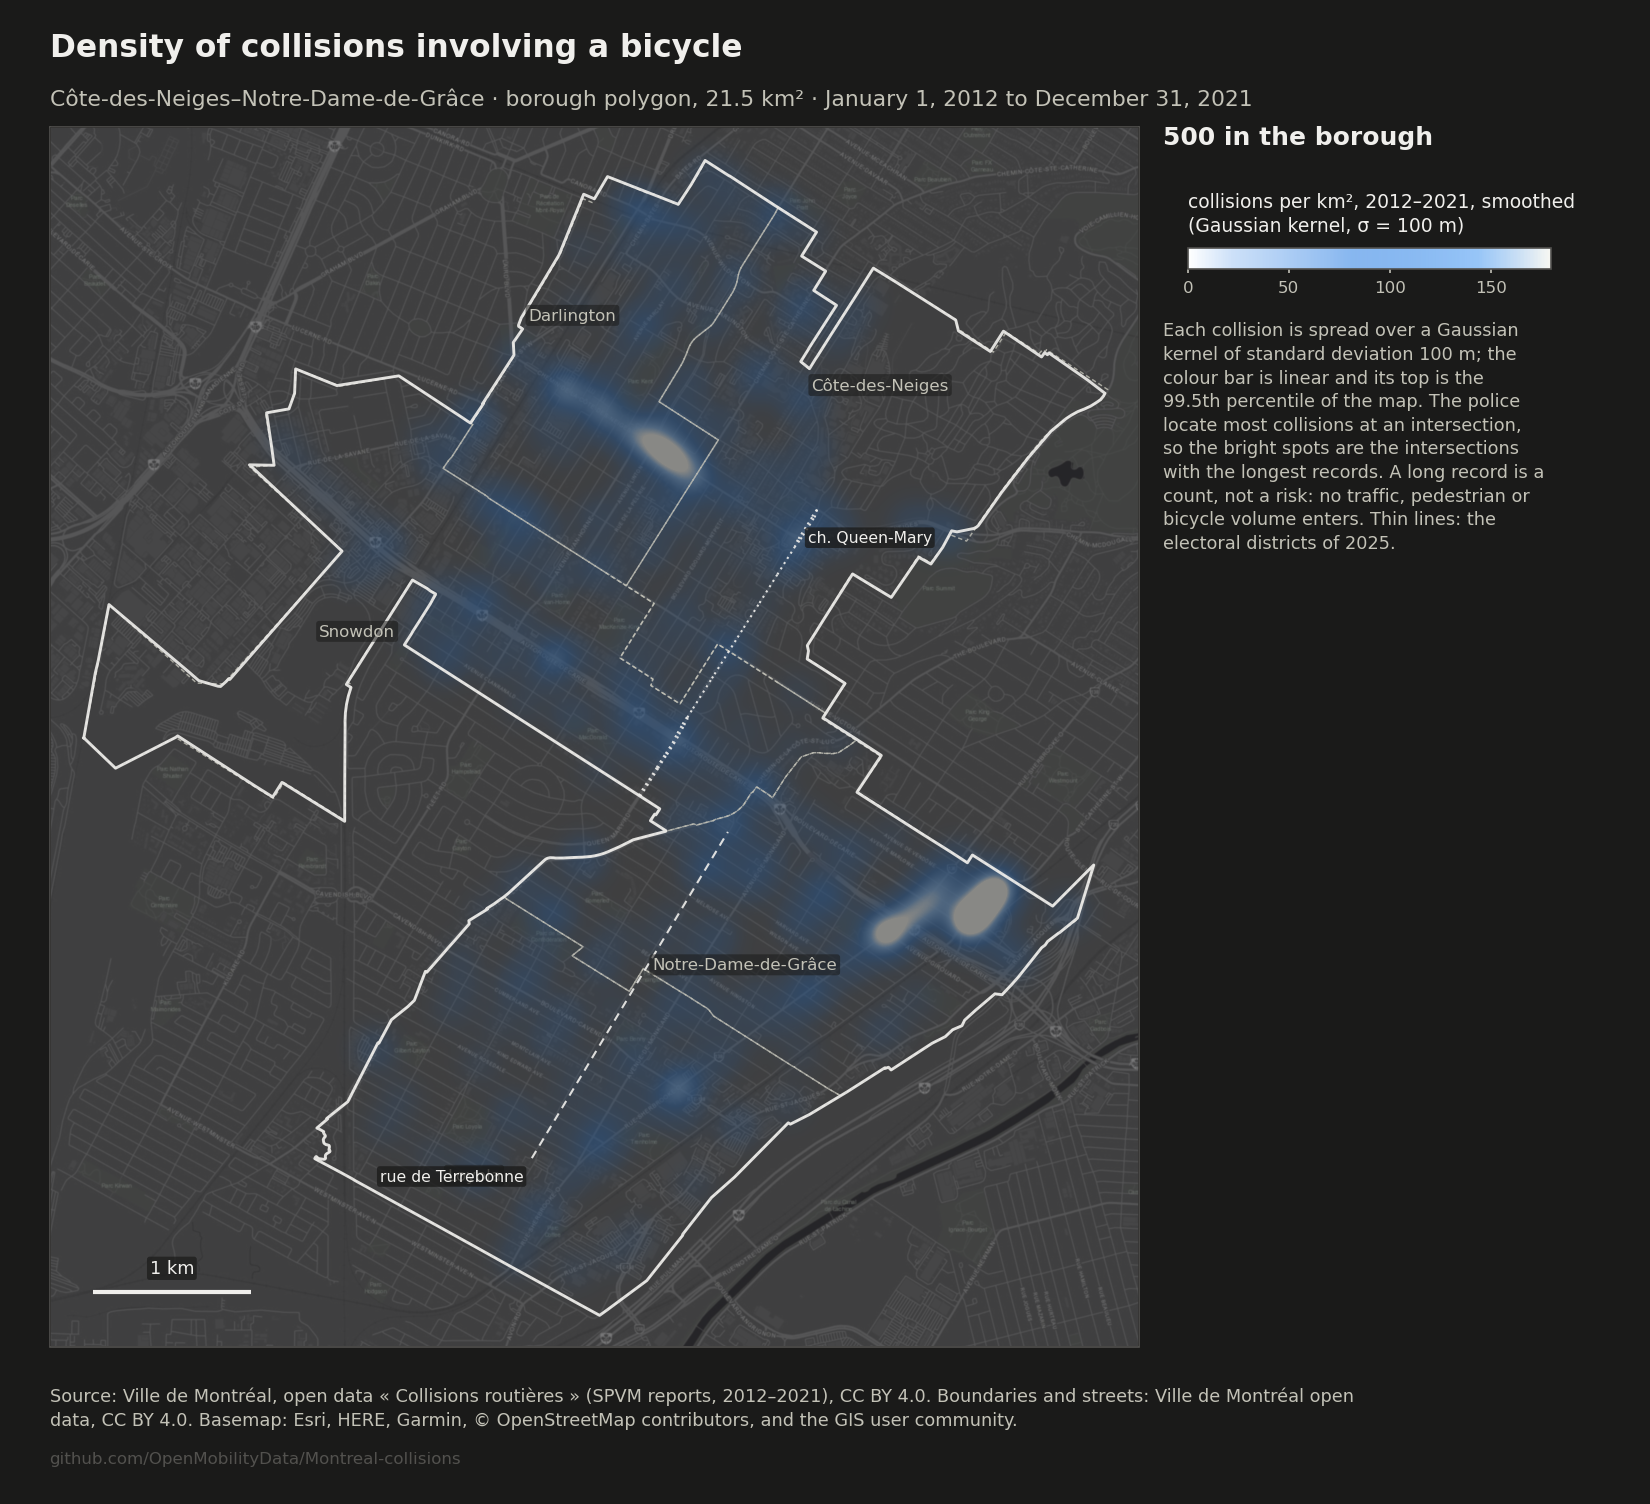
\includegraphics[width=\linewidth,height=0.84\textheight,keepaspectratio]{../derived/figures/cdn-ndg-maps/cdn_ndg_bike_heat_en.png}\end{center}
\end{frame}

\begin{frame}{Bicycles: collisions with a death or a severe injury}
\begin{center}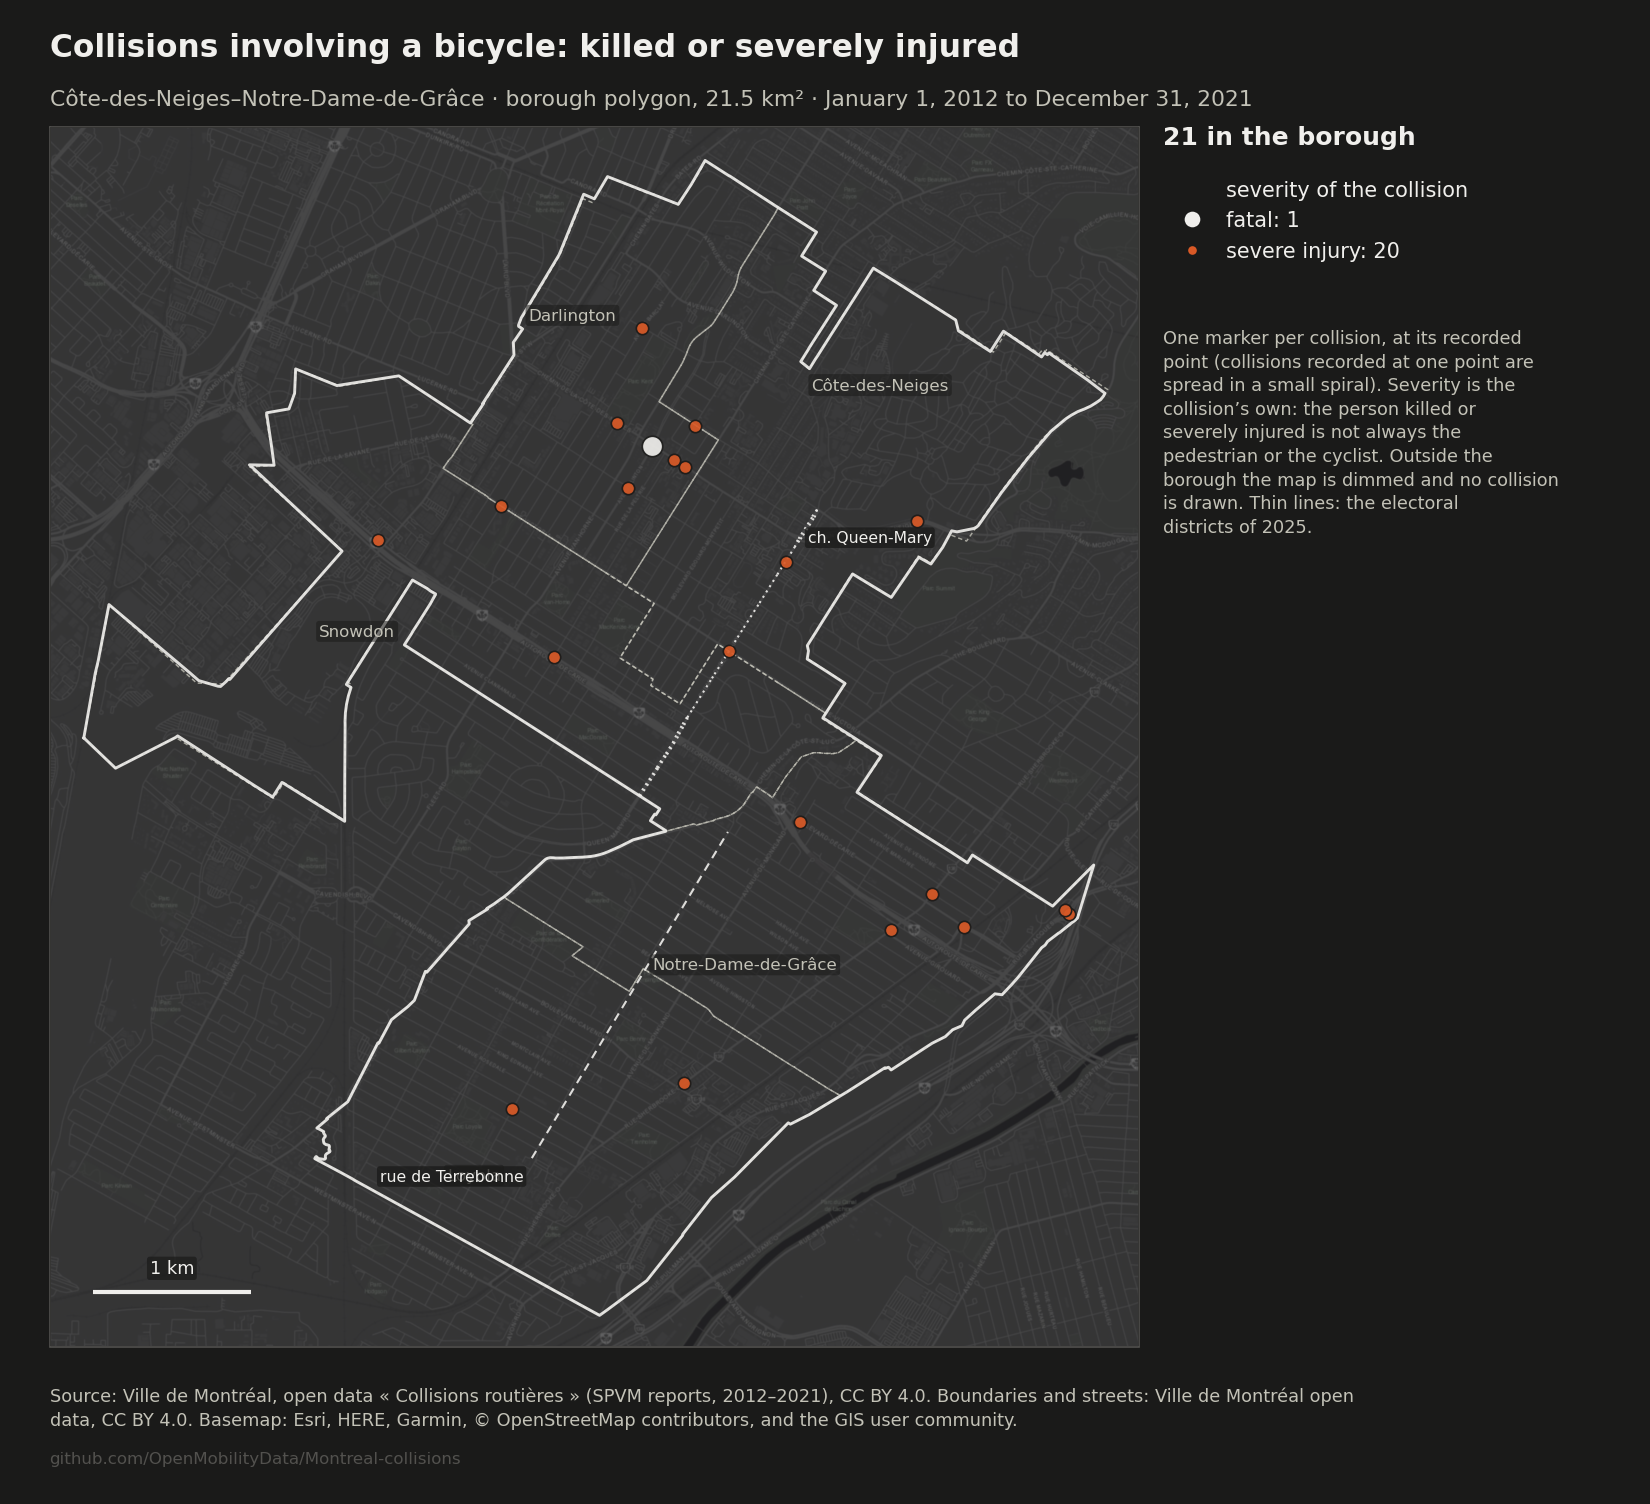
\includegraphics[width=\linewidth,height=0.84\textheight,keepaspectratio]{../derived/figures/cdn-ndg-maps/cdn_ndg_bike_serious_en.png}\end{center}
\end{frame}

\begin{frame}{By the other vehicle}
\small
\begin{tabular}{@{}lrrrrr@{}}\toprule
 & collisions & fatal & severe & light & severe or fatal \\\midrule
\multicolumn{6}{@{}l}{\textbf{With a pedestrian victim}} \\
car or light truck & 878 & 9 & 65 & 804 & 8~\% \\
heavy truck or tractor-trailer & 26 & 5 & 4 & 17 & 35~\% \\
bus or minibus & 30 & 1 & 3 & 26 & 13~\% \\
other or none recorded & 68 & 1 & 6 & 61 & 10~\% \\
\midrule
\multicolumn{6}{@{}l}{\textbf{Involving a bicycle}} \\
car or light truck & 446 & 1 & 16 & 325 & 4~\% \\
heavy truck or tractor-trailer & 8 & 0 & 2 & 6 & 25~\% \\
bus or minibus & 12 & 0 & 1 & 10 & 8~\% \\
other or none recorded & 34 & 0 & 1 & 25 & 3~\% \\
\bottomrule
\end{tabular}
\medskip
\begin{itemize}\setlength\itemsep{4pt}
\item Order of precedence when several vehicles are recorded: heavy truck, bus, car or light truck.
\item Collisions, by the collision's severity. The heavy-vehicle rows are small: read them as counts, not as rates.
\item Bicycle rows include collisions with property damage only, so the four severity columns do not sum to the first.
\end{itemize}
\end{frame}

\begin{frame}{The intersections with the longest records}
\begin{center}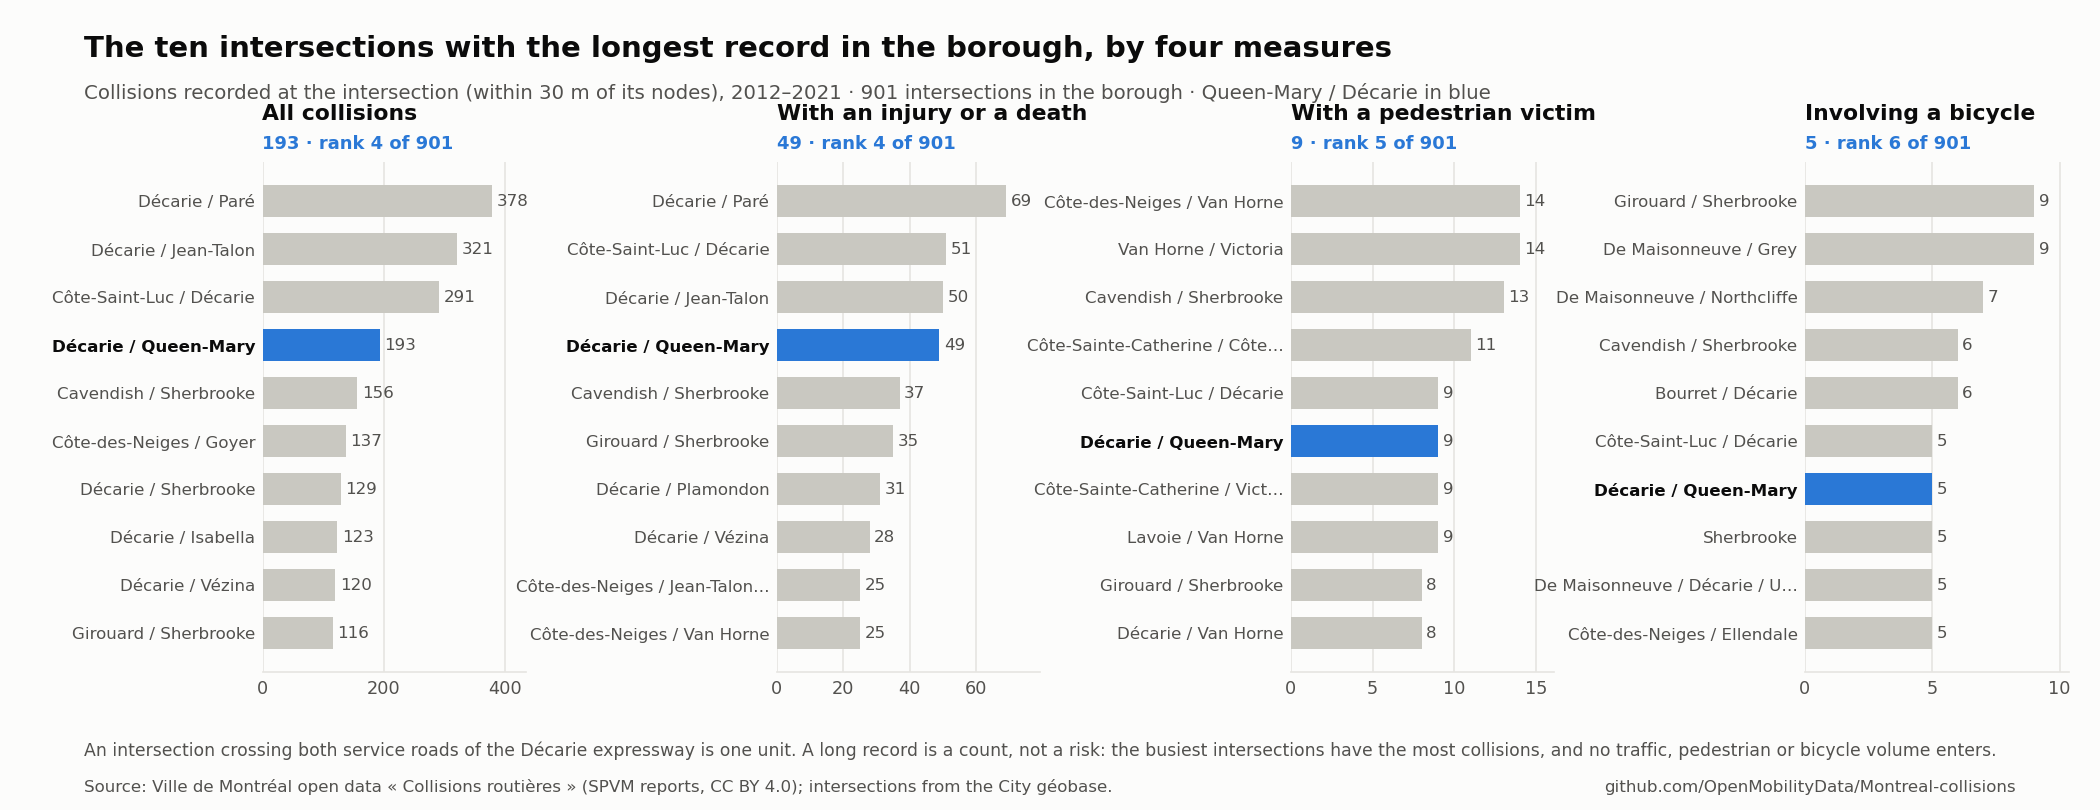
\includegraphics[width=\linewidth,height=0.8\textheight,keepaspectratio]{../derived/figures/cdn-ndg-charts/cdn_ndg_intersections_en.png}\end{center}
\end{frame}

\begin{frame}{Chemin Queen-Mary}
\begin{center}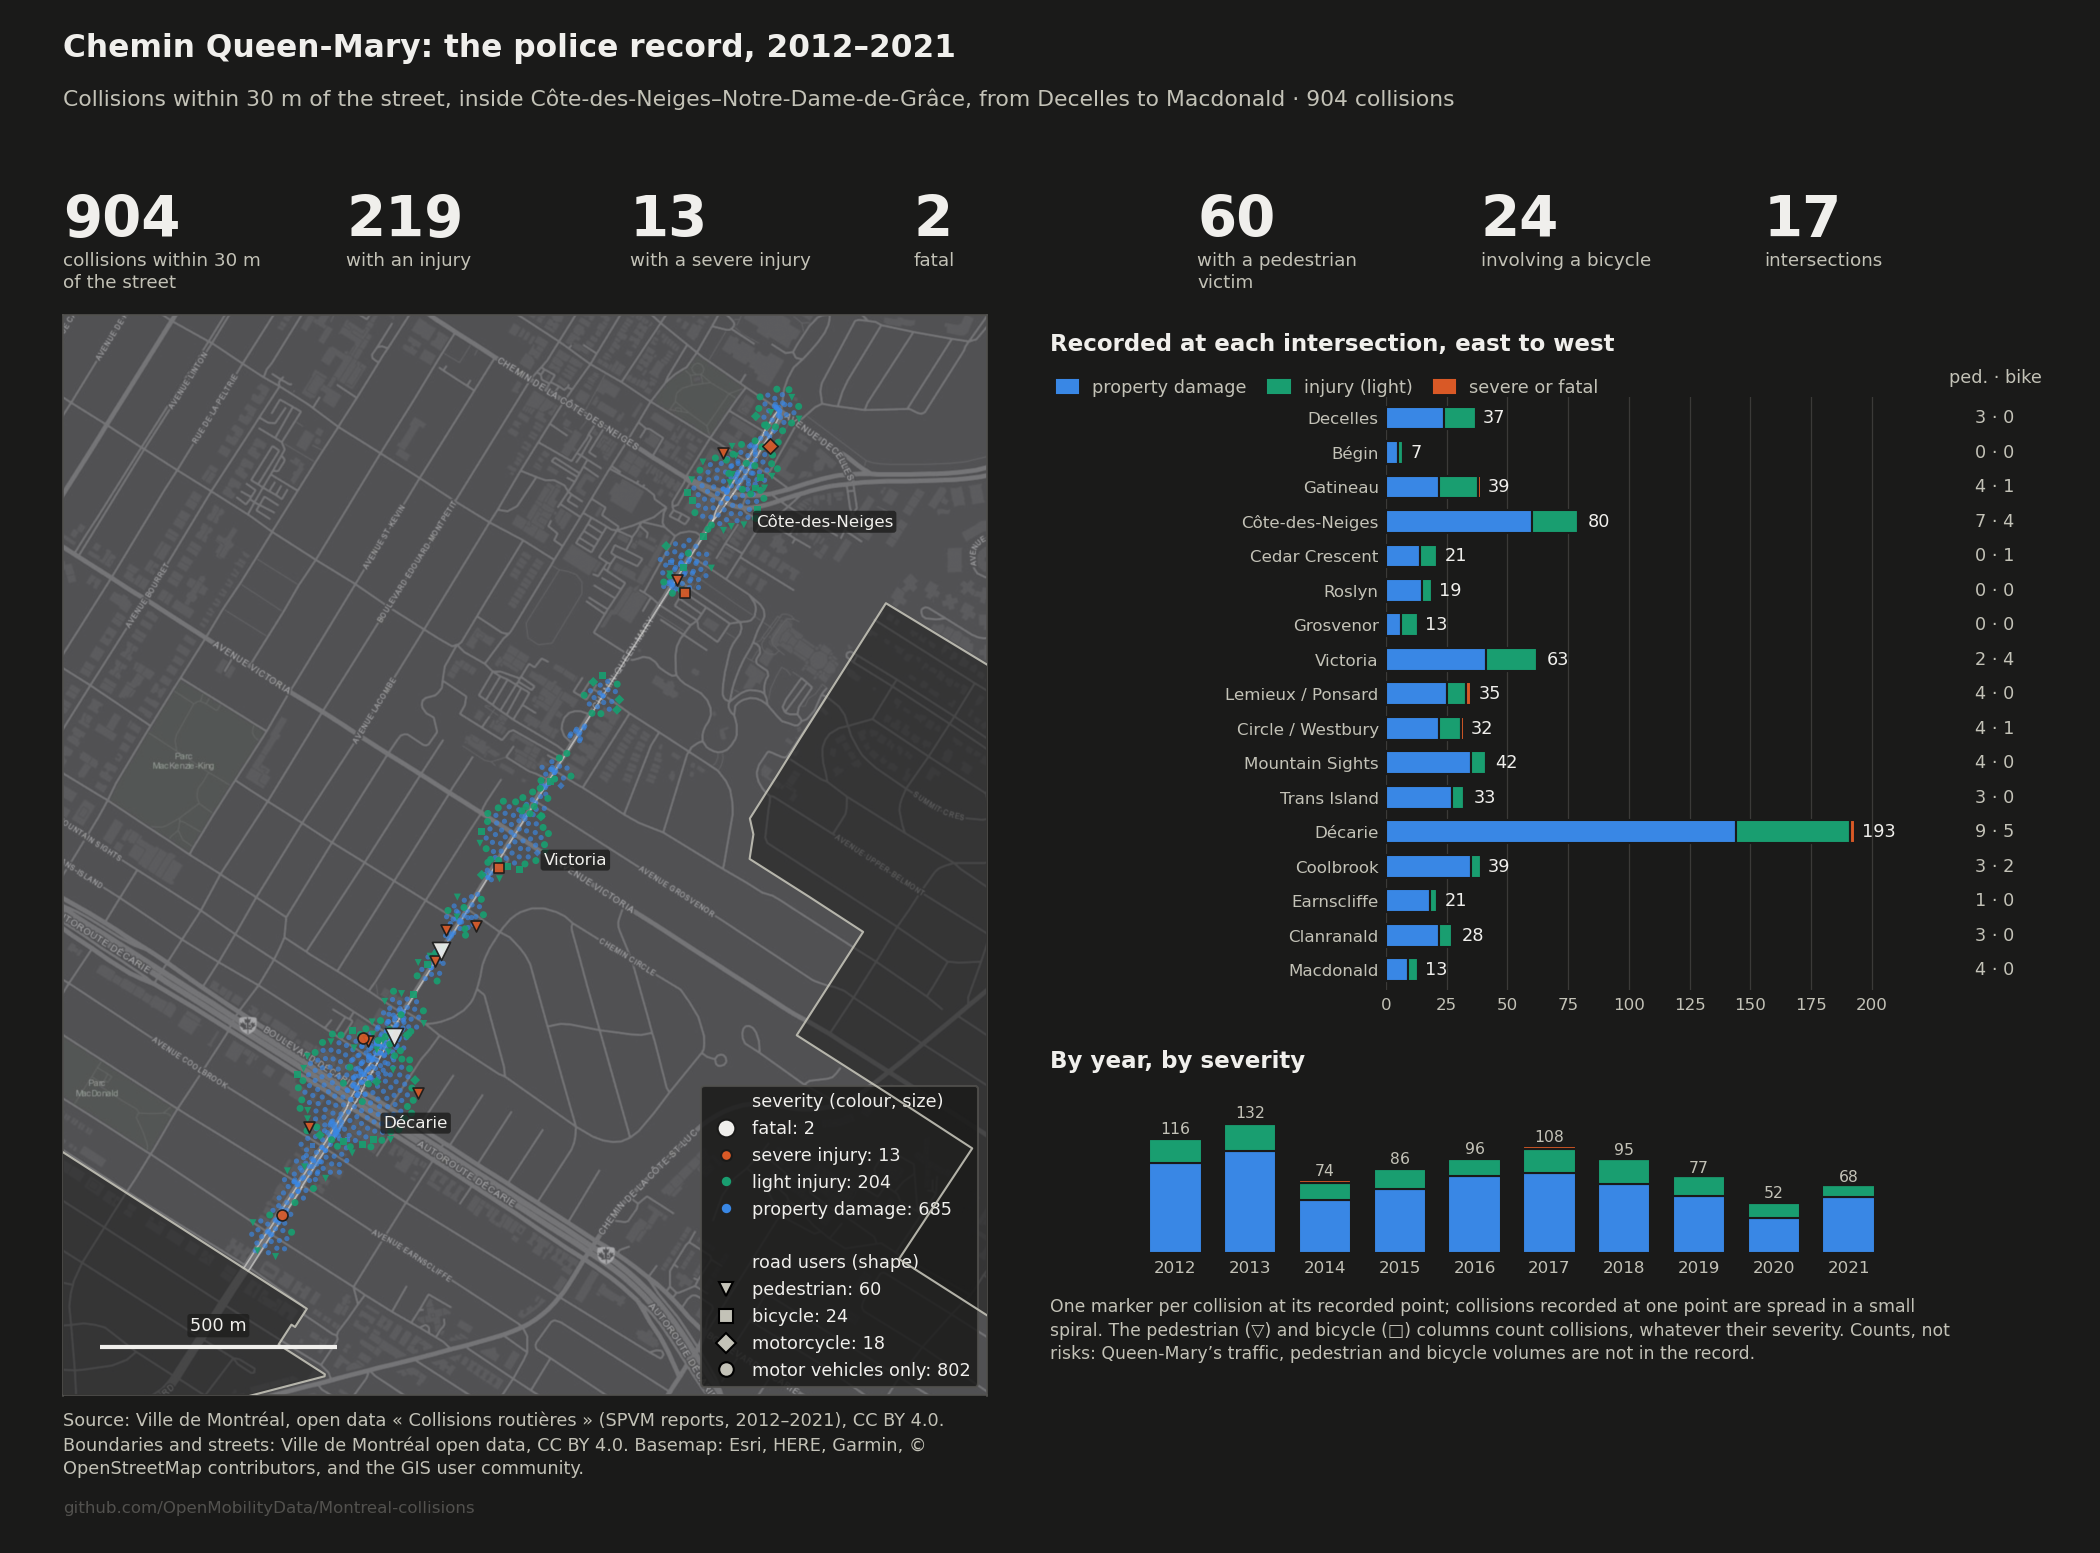
\includegraphics[width=\linewidth,height=0.86\textheight,keepaspectratio]{../derived/figures/queen-mary/overview_queen_mary_corridor_en.png}\end{center}
\end{frame}

\begin{frame}{Queen-Mary / Décarie}
\begin{center}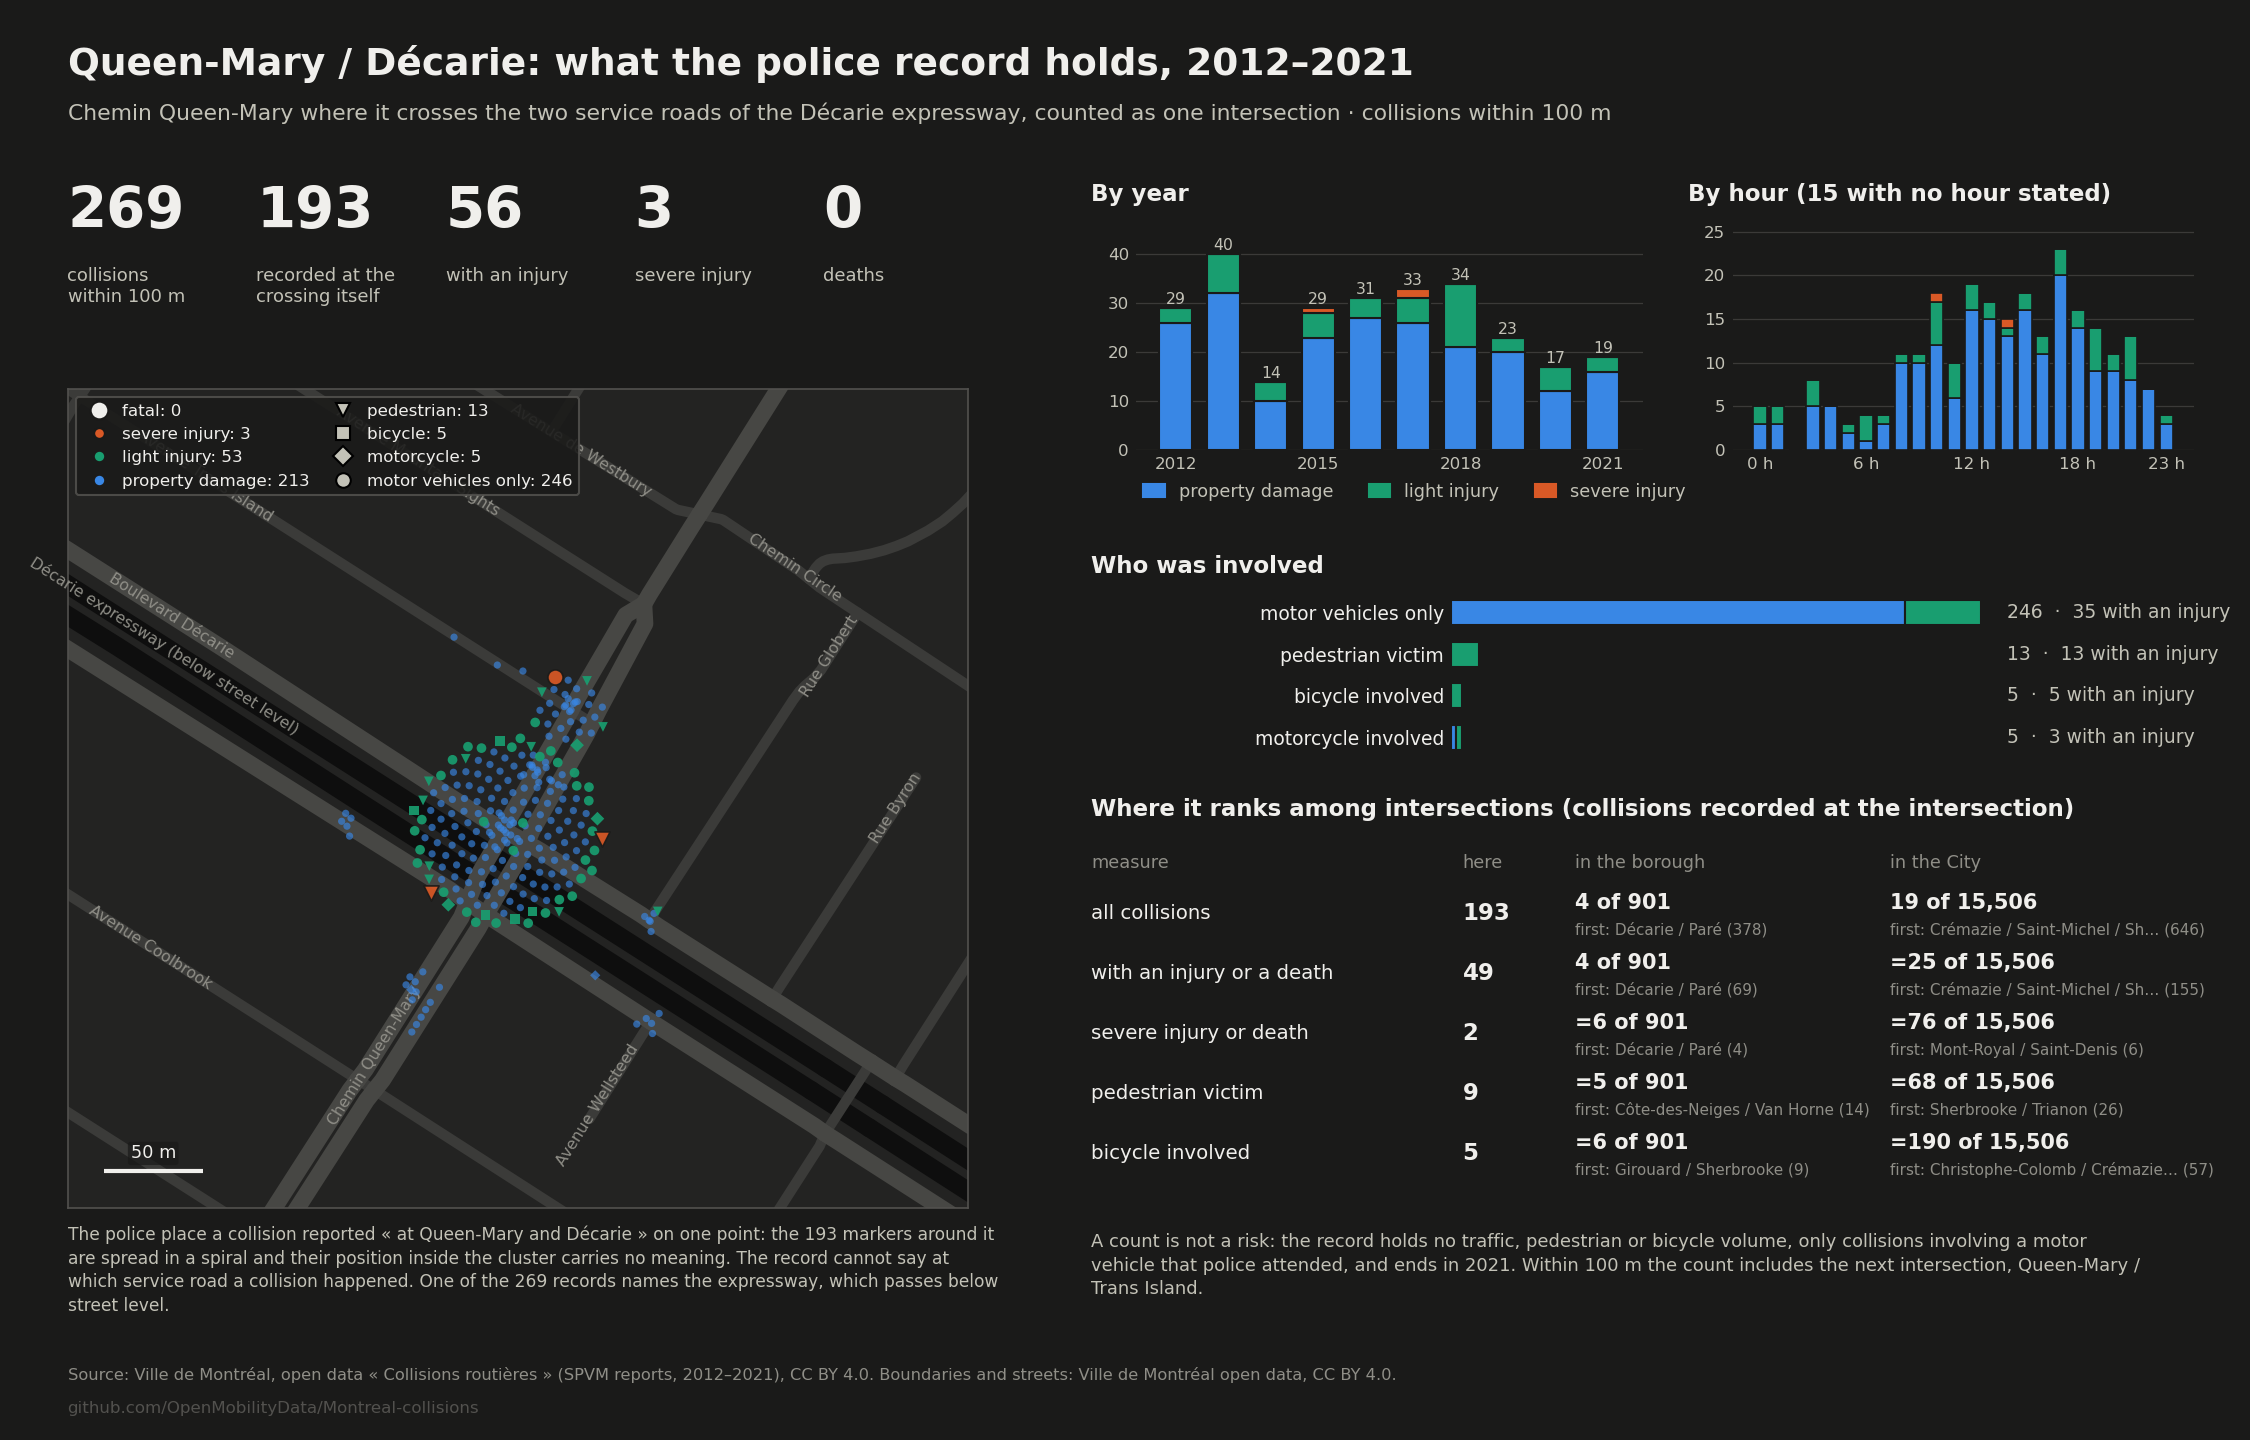
\includegraphics[width=\linewidth,height=0.86\textheight,keepaspectratio]{../derived/figures/queen-mary-decarie-overview/overview_queen_mary_decarie_en.png}\end{center}
\end{frame}

\begin{frame}{Rue de Terrebonne: every collision within 25 m of the lane's axis}
\begin{center}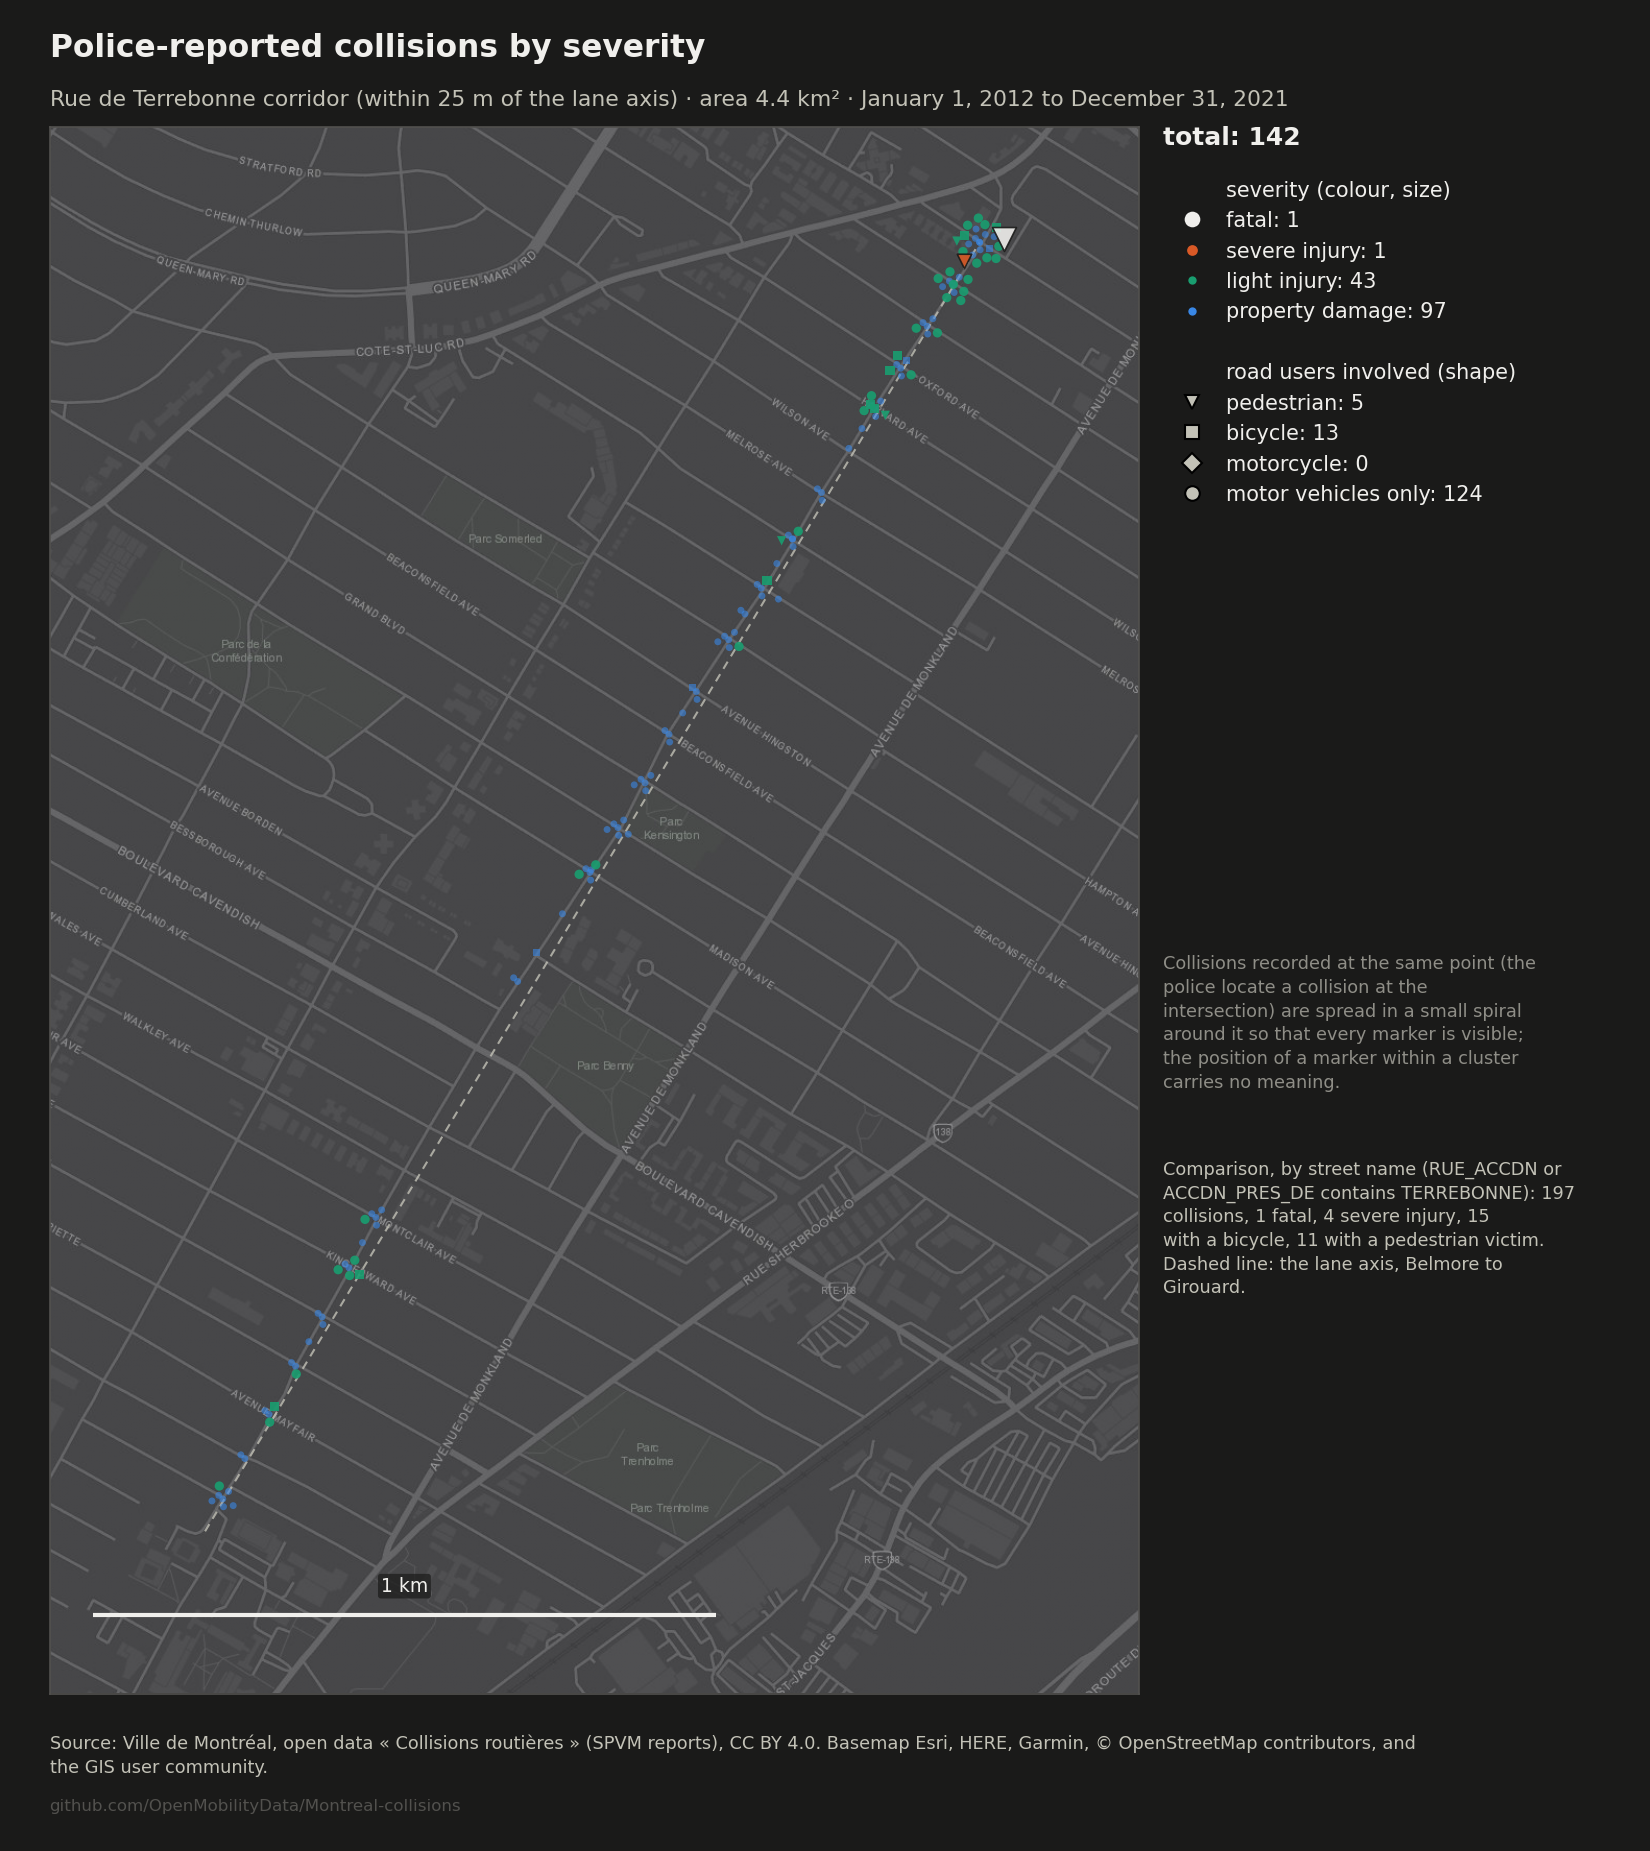
\includegraphics[width=\linewidth,height=0.84\textheight,keepaspectratio]{../derived/figures/maps/corridor_severity_en.png}\end{center}
\end{frame}

\begin{frame}{Rue de Terrebonne: collisions involving a bicycle or a pedestrian victim}
\begin{center}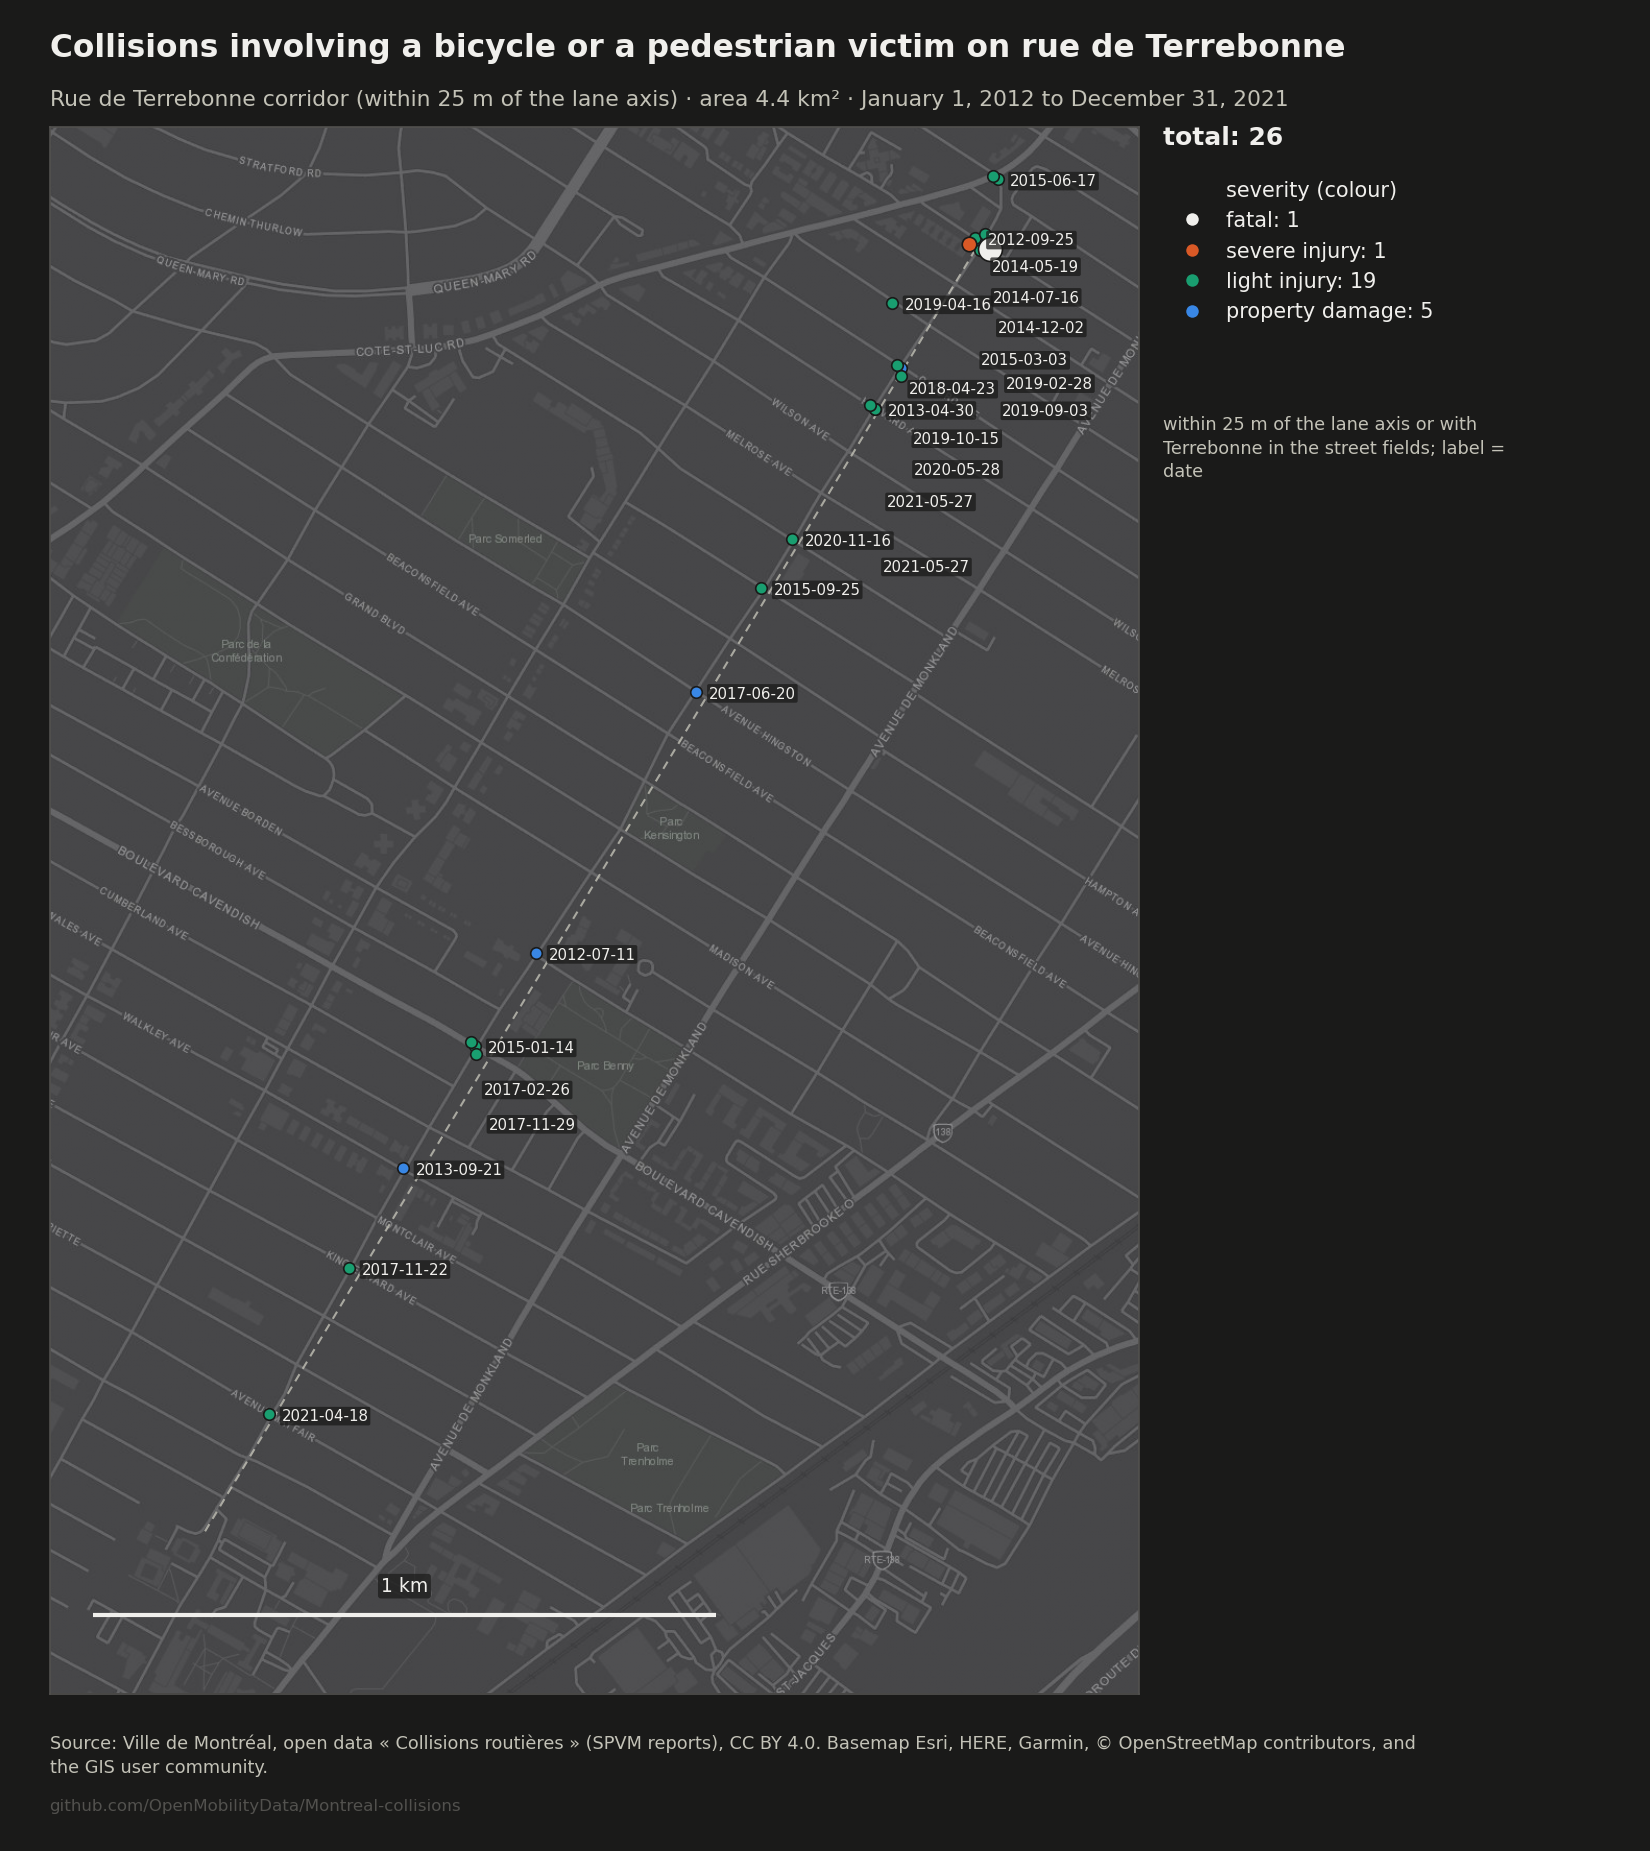
\includegraphics[width=\linewidth,height=0.84\textheight,keepaspectratio]{../derived/figures/maps/corridor_vru_en.png}\end{center}
\end{frame}

\begin{frame}{Rue de Terrebonne: what can and cannot be said}
\begin{itemize}\setlength\itemsep{6pt}
\item The record predates the protected lane (built 2024): it describes the street as it was.
\item Terrebonne / Girouard, collisions recorded at the intersection: 23 (rank 114 of 901 in the borough), 13 with an injury (rank 44), 3 with a pedestrian victim, 3 involving a bicycle.
\item Rates per crossing (next slide) exist only where the City counted, on a few days. For bicycles the counts differ by more than an order of magnitude between visits, so no single rate is quotable: each figure goes with its interval and its exposure method.
\item City-wide, an earlier fatal collision at the same place was not a precursor of a cyclist's death; the volume of the earlier record was, in the aggregate, and it points to the busy tenth of the city, not to a place.
\end{itemize}
\end{frame}

\begin{frame}{Terrebonne / Girouard and rue Sherbrooke: collisions per million crossings}
\begin{center}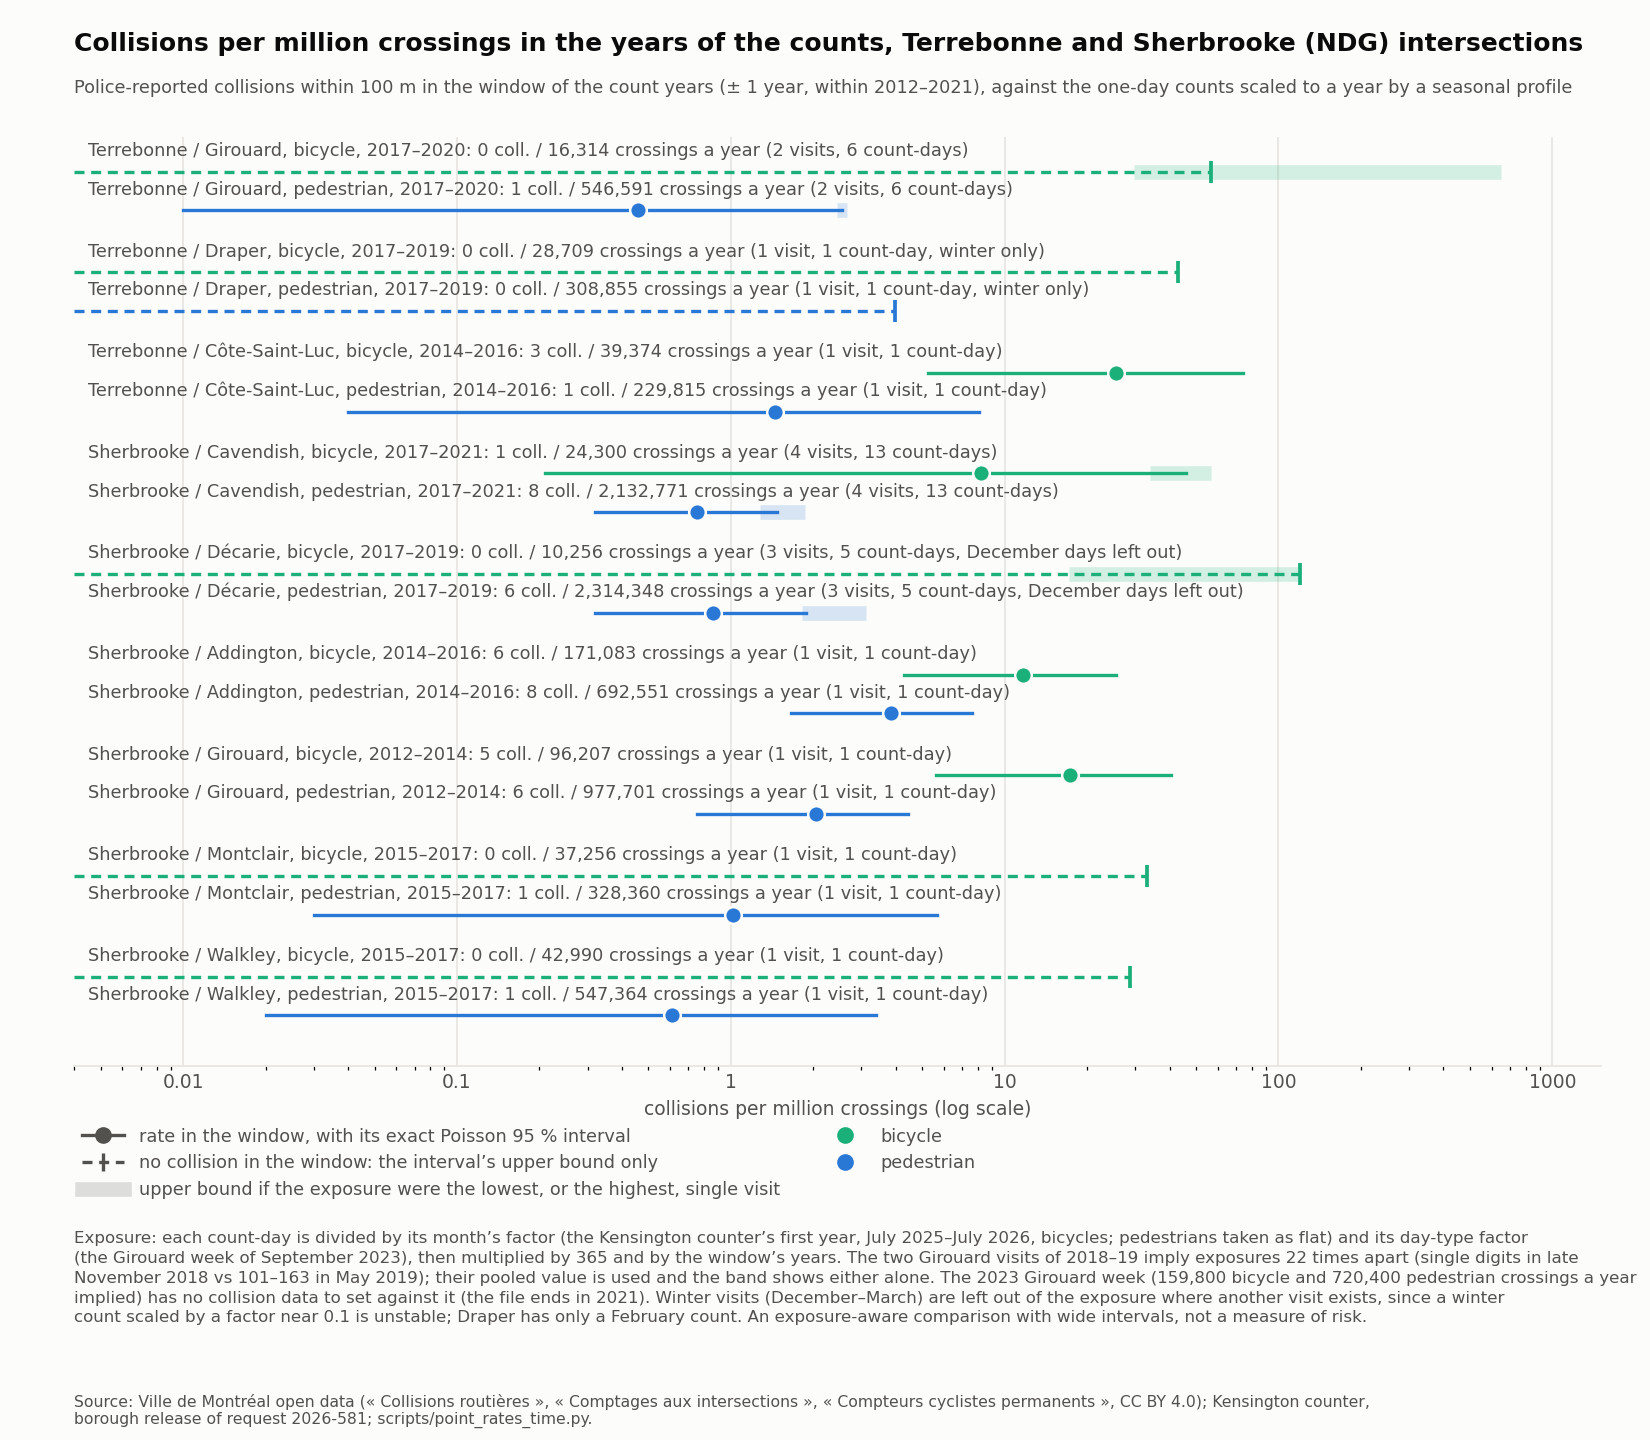
\includegraphics[width=\linewidth,height=0.84\textheight,keepaspectratio]{../derived/figures/charts/point_rates_time_en.png}\end{center}
\end{frame}

\begin{frame}{Definitions}
\small
\begin{itemize}\setlength\itemsep{4pt}
\item \textbf{Borough and districts.} The City's administrative-limits polygon and its electoral districts of 2025 (open data). A collision belongs where its recorded point falls.
\item \textbf{Severity} is the collision's own (fatal, severe injury, light injury, property damage). \textbf{Pedestrian}: at least one pedestrian victim. \textbf{Bicycle}: a bicycle involved or a cyclist victim.
\item \textbf{Denominators.} Street length: City géobase, local, collector and arterial streets, a divided street counted once per carriageway. Residents: 2021 Census, dissemination areas placed by a point inside each.
\item \textbf{Intersection.} Géobase nodes where two street names or three segment ends meet; nodes within 30 m are one intersection, and so are same-name units within 120 m (a street crossing both Décarie service roads). 901 in the borough, 15{,}506 in the City.
\item \textbf{Two counts.} Recorded at the intersection: within 30 m of its nodes, each collision given to one intersection. Within 100 m: every collision in that radius, shared between neighbours.
\item \textbf{Queen-Mary / Décarie.} One intersection. Of 269 collisions within 100 m, 193 sit on the crossing's recorded point; 37 are coded on a ramp, collector or service road. The record cannot separate the two service roads.
\end{itemize}
\end{frame}

\begin{frame}{Limits, and where everything is}
\small
\begin{itemize}\setlength\itemsep{5pt}
\item No exposure measure by borough, street or intersection: every figure here is a count or a count against residents or street length, never a risk per trip.
\item 2012--2021 only; no age; police-attended collisions with a motor vehicle only.
\item Small numbers: a rank built on fewer than ten events moves with one collision.
\item Recorded points are approximate: 19{,}196 rows of the file are flagged imprecise, among them every collision recorded at a service-road crossing.
\item Not done: any before-and-after of a street change; any comparison of intersections by traffic volume.
\end{itemize}
\medskip
Code, tables and figures (English and French): \texttt{github.com/OpenMobilityData/Montreal-collisions}\\
Data: Ville de Montréal, « Collisions routières », géobase, administrative limits, electoral districts (CC BY 4.0); Statistics Canada, 2021 Census. Basemap: Esri, HERE, Garmin, © OpenStreetMap contributors.
\end{frame}
\end{document}
